\documentclass{article}
\PassOptionsToPackage{numbers,sort&compress}{natbib}
\usepackage[eandd]{neurips_2026}

\usepackage[utf8]{inputenc}
\usepackage[T1]{fontenc}
\usepackage{booktabs}
\usepackage{longtable}
\usepackage{array}
\usepackage{tabularx}
\usepackage{multirow}
\usepackage[table]{xcolor}
\usepackage{amsmath,amssymb}
\usepackage{hyperref}
\usepackage{xurl}
\usepackage{fancyvrb}
\usepackage{graphicx}
\usepackage{placeins}
\usepackage[most]{tcolorbox}

\newtcolorbox{modelbox}{
  colback=gray!6,
  colframe=gray!35,
  boxrule=0.35pt,
  arc=1.2pt,
  left=4pt,
  right=4pt,
  top=3pt,
  bottom=3pt,
  before skip=4pt,
  after skip=4pt,
  breakable,
  enhanced
}
\hypersetup{
  colorlinks=true,
  linkcolor=blue!50!black,
  urlcolor=blue!50!black,
  citecolor=blue!50!black
}

\newcommand{\code}[1]{\texttt{#1}}
\newcolumntype{Y}{>{\raggedright\arraybackslash}X}
\newcommand{\missingmetric}{n/a}
\newcommand{\yesmark}{\textcolor{NightTrapGreen}{\checkmark}}
\newcommand{\nomark}{\textcolor{red!75!black}{$\times$}}
\definecolor{NightTrapBlue}{HTML}{173C8F}
\definecolor{NightTrapBlueBack}{HTML}{F1F5FF}
\definecolor{NightTrapGreen}{HTML}{0B7A2A}
\definecolor{NightTrapGreenBack}{HTML}{F0FAF2}
\definecolor{NightTrapGold}{HTML}{7A6A20}
\definecolor{NightTrapGoldBack}{HTML}{FFF9E8}
\definecolor{NightTrapGray}{HTML}{F2F2F2}
\newtcolorbox{appendixbox}[2][]{
  enhanced,
  breakable,
  colback=#2!6,
  colframe=#2!85!black,
  colbacktitle=#2!85!black,
  coltitle=white,
  boxrule=0.9pt,
  arc=2mm,
  left=5pt,
  right=5pt,
  top=5pt,
  bottom=5pt,
  fonttitle=\bfseries,
  #1
}
\emergencystretch=6em

\title{NightTrap: A Workflow-Structured Benchmark for Night Camera-Trap Triage in Ecological Monitoring}
\author{Anonymous submission}
\date{}

\begin{document}
\maketitle

\begin{abstract}
Camera traps are central to biodiversity monitoring and conservation, but night deployments produce large volumes of infrared and low-light events that still require human review. We introduce \textbf{NightTrap}, a workflow-structured benchmark for night camera-trap triage in ecological monitoring. NightTrap is built from \textbf{68,187 night events across 2,902 camera sites} and evaluates five review decisions: whether visual evidence is usable, whether an event is safely empty, which species is present, how many animals are visible, and whether the event should enter a human review queue. The benchmark separates recognition accuracy from operational triage metrics, including queue-front enrichment and recall-constrained safe auto-pass. Experiments with open-source vision-language models, supervised vision baselines, lightweight rankers, and camera-trap screening methods show that current models can enrich human review queues but cannot safely replace expert inspection. NightTrap also exposes a key deployment risk: site-history context can support review routing, but it can also create shortcut behavior unless Visual Only, Context Only, Combined, and Shortcut Check settings are reported together.
\end{abstract}

\section{Introduction}

% 相机陷阱是野生动物监测中的重要工具。它可以长期部署在野外，无需人工值守即可捕捉动物活动。然而，相机陷阱并没有消除人工工作量，而是把大量工作转移到了后端审核阶段。研究人员仍然需要过滤无效事件、判断图像是否可判读、识别动物、估计数量，并决定哪些事件应当更早交由人工查看。
Camera traps are an important tool for wildlife monitoring. They can be deployed in the field for long periods and capture animal activity without continuous human presence. However, camera traps do not remove human labor. They shift much of the work to downstream review, where researchers must filter invalid events, assess image usability, identify animals, estimate counts, and decide which events need human review.

% 夜间相机陷阱数据使这一流程更加困难。相比白天图像，夜间图像常常缺少颜色和纹理信息，并依赖红外或低照度成像。动物可能只呈现模糊轮廓；近距离动物可能被红外打白；远距离动物可能过暗而难以识别；运动中的动物也更容易模糊。因此，夜间审核的第一个问题往往不是“这是什么动物”，而是“这张图是否有足够视觉证据支持可靠判断”。
Night camera-trap data makes this workflow harder. Compared with daytime images, night images often lose color and texture information and rely on infrared or low-light imaging. Animals may appear only as weak silhouettes; nearby animals may be overexposed by infrared illumination; distant animals may be too dark to identify; and moving animals can be blurred. For this reason, the first question in night review is often not ``what species is this?'', but ``is there enough visual evidence to make a reliable judgment?''

% 已有相机陷阱 benchmark 已经研究动物存在判断、空图过滤、物种分类、数量估计和跨相机点位泛化。这些任务重要，但它们通常作为孤立识别任务评估。真实夜间审核更接近一个流程：先判断图像证据是否可用，再判断是否为空，再识别动物类别和数量，最后判断哪些事件应当排到人工审核队列前端。
Prior camera-trap datasets, challenges, and recognition pipelines have studied animal presence, empty filtering, species classification, counting, and generalization to unseen camera sites \citep{norouzzadeh2017snapshot,beery2019iwildcam,koh2021wilds,schneider2018camera,choinski2021first}. These tasks are important, but they are often evaluated as isolated recognition tasks. Real night review is sequential: reviewers first decide whether evidence is usable, then whether the event is empty, then which species and count are present, and finally which events require human attention rather than being deprioritized for later review. NightTrap follows this order, but the main results evaluate the decision points separately rather than making one all-in-one score the central result. Table~\ref{tab:related-work-matrix} summarizes this coverage gap.

\begin{table}[t]
\centering
\caption{Coverage comparison with related benchmarks. ``Partial'' means the work touches the item but does not make it a core task; a red cross means the item is not covered.}
\label{tab:related-work-matrix}
\small
\setlength{\tabcolsep}{3pt}
\begin{tabularx}{\textwidth}{p{2.7cm} *{6}{>{\centering\arraybackslash}X}}
\toprule
Work & Night data & Image usability / filtering & Species & Count & Behavior & Needs review \\
\midrule
Camera-trap recognition benchmarks & \yesmark & partial & \yesmark & partial & \nomark & \nomark \\
Animal-Bench & \nomark & \nomark & partial & \nomark & \yesmark & \nomark \\
Animal Kingdom & \nomark & \nomark & partial & \nomark & \yesmark & \nomark \\
MammalNet & \nomark & \nomark & \yesmark & \nomark & partial & \nomark \\
NightTrap (ours) & \yesmark & \yesmark & \yesmark & \yesmark & \nomark & \yesmark \\
\bottomrule
\end{tabularx}
\end{table}

% 为了启发这一流程设计，我们进行了面向生态监测相关人群的小规模问卷调研。问卷问题和完整统计放在附录。问卷共收集 17 份有效身份信息，其中 52.94% 为高校/科研院所在校学生，5.88% 为政府保护部门或保护区管理人员，11.76% 为民间保护组织工作人员/管理者，11.76% 为长期志愿者或独立研究者，17.65% 为其他相关身份。70.59% 的受访者表示经常或偶尔使用自动监测设备，另外 29.41% 虽未使用但有兴趣了解。
To motivate the workflow design, we conducted a small questionnaire targeting people connected to ecological monitoring; the full instrument and statistics are in the appendix. The responses support the workflow framing: respondents emphasized poor image quality, excessive data volume, counting difficulty, and expert confirmation rather than full automation. We use the questionnaire only as task-design motivation, not as large-scale user-study evidence.

% 小规模问卷提示，受访者遇到的主要困难与完整审核流程一致，而不是只集中在“识别物种”一个问题上。在监测数据处理困难中，83.33% 的受访者选择“照片质量差，难以辨认”，58.33% 选择“数据量太大，人工看不过来”，58.33% 选择“想统计动物数量，但不知道怎么避免重复计数”，50.00% 选择“想知道动物行为，但缺乏系统方法”。这些回答用于启发任务组织，而不是作为大规模用户研究证据。
% 受这些调查结果启发，NightTrap 将夜间相机陷阱审核组织为五个任务：Image usability filtering、Empty-event filtering、Species classification、Count-bin classification 和 Needs-review recommendation。它们分别对应问卷中反复出现的审核环节：低质量图像判断、无效或空触发过滤、物种识别、数量估计，以及在有限人工审核预算下发现需要人工审核的事件。空图过滤、动物分类和数量估计本身并非全新任务。NightTrap 的贡献是将这些已有但分散的环节组织为一个夜间审核流程，并评估模型能否协助人工审核。
Motivated by these responses, NightTrap organizes night camera-trap review into five tasks: Image usability filtering, Empty-event filtering, Species classification, Count-bin classification, and Needs-review recommendation. These tasks correspond to recurring review steps in the questionnaire: judging low-quality visual evidence, filtering invalid or empty triggers, identifying species, estimating counts, and deciding which events require human review under limited review budgets. Empty filtering, species classification, and counting are not claimed as new tasks. The contribution of NightTrap is to make these established but scattered steps comparable under one night-review setting and to evaluate whether models can assist human review.

% 本文实验也围绕这一需求展开：模型能否完成基础筛查和识别，并在有限人工审核预算下把更需要人工查看的事件排到前面。我们因此同时报告分类指标、排序指标和 safe auto-pass 指标，以区分“协助审核排序”和“安全减少人工工作量”这两种不同能力。
Our experiments follow the same need: can models perform basic filtering and recognition, and then recommend which events need human attention under limited review budgets? We therefore report classification metrics, review-score ranking metrics, and safe auto-pass metrics, so that review assistance through queue ordering can be distinguished from safe workload reduction.

% 总结起来，本文的主要贡献如下：
NightTrap contributes a frozen benchmark of 68,187 night events across 2,902 camera sites, five review-facing tasks, and a Task 5 needs-review setting that separates queue ordering from recall-constrained safe auto-pass. We evaluate open-source VLMs, supervised vision baselines, lightweight rankers, camera-trap screening methods, and closed-source reference rows. The results show long-tail species failures, the importance of image usability, limited safe auto-pass, shortcut risk from site context, and the need to report decision points separately rather than relying on one all-in-one score.
\section{Related Work}

\subsection{Existing Camera-Trap Datasets and Benchmarks}

% 相机陷阱数据集。早期相机陷阱 benchmark 主要关注动物存在判断、物种识别、计数和跨相机泛化。Snapshot Serengeti 证明了深度学习可以在大规模相机陷阱图像上进行自动动物识别、计数和描述；Caltech Camera Traps、iWildCam 和 WILDS-iWildCam 进一步强调，相机陷阱数据存在显著的点位偏移和背景记忆问题，因此不能只依赖随机划分评估模型。
Prior camera-trap datasets, challenges, and recognition pipelines mainly focus on animal presence, species recognition, counting, and cross-camera generalization. Snapshot Serengeti showed that deep learning can identify, count, and describe wild animals in large camera-trap collections \citep{norouzzadeh2017snapshot}. Caltech Camera Traps, iWildCam, and WILDS-iWildCam further emphasize site-level distribution shift and background memorization risks, making random splits insufficient for deployment-oriented evaluation \citep{beery2019iwildcam,koh2021wilds}. Detector and classifier pipelines are also central to practical camera-trap review, because they can filter empty images, localize animals, and support downstream classification \citep{schneider2018camera,choinski2021first,gomez2016towards,beery2019pipeline}. NightTrap builds on this line of work, but evaluates the surrounding night-review decisions in addition to species recognition.

% 检测和分类。另一类工作将相机陷阱审核转化为检测或分类问题。检测模型可以过滤空图、定位动物并支持后续分类；分类模型可以识别常见物种并减少人工标注量。这些工作对生态监测非常重要，但任务通常以单图识别、检测或分类为核心，缺少对夜间审核流程中“图像是否可判读”“事件是否需要优先人工查看”等前后衔接环节的统一建模。
Recent representation models such as CLIP and DINOv2 make retrieval or linear-probe baselines attractive for camera-trap species recognition, while supervised backbones such as ViT and ConvNeXt provide task-specific visual baselines \citep{radford2021clip,oquab2023dinov2,dosovitskiy2021vit,liu2022convnext}. Long-tail recognition work motivates reporting balanced metrics rather than only aggregate accuracy \citep{gupta2019lvis,vanhorn2018inaturalist,lin2017focalloss}. These methods are complementary to NightTrap: they are important baselines for the recognition steps, while the benchmark asks how recognition fits into triage decisions around usable evidence, empty screening, count bins, and review queues.



\subsection{Animal-Centric Vision and Multimodal Benchmarks}

% 动物视觉理解 benchmark。近年来的动物中心 benchmark 覆盖了更丰富的动物视觉理解任务。例如 Animal-Bench 评估多模态视频模型的动物中心理解能力，Animal Kingdom 关注动物行为理解，MammalNet 提供大规模哺乳动物识别和行为理解视频 benchmark。这些数据集拓展了动物视觉理解的范围，但它们通常不面向相机陷阱审核流程，也不将空图过滤、坏图过滤、数量分档和优先审核排序作为统一评估链条。
Animal-Bench, Animal Kingdom, and MammalNet broaden animal visual understanding beyond static species recognition, including video and behavior tasks \citep{jing2024animalbench,ng2022animalkingdom,chen2023mammalnet}. These benchmarks are valuable, but they are not designed around camera-trap review triage. In particular, they do not combine empty filtering, image usability filtering, count-bin classification, and needs-review recommendation in the same night-review setting.



\subsection{Camera-Trap Review Systems and Automation Methods}

% 自动审核系统。相机陷阱审核系统通常将检测器、分类器和人工复核结合起来，以减少空图和低价值图像带来的人工负担。典型流程包括先检测动物，再分类物种，最后将低置信度或高风险样本交给人工确认。这些系统说明实际部署并不追求模型完全替代专家，而是追求减少人工负担和提高审核效率。
Camera-trap review systems often combine detectors, classifiers, and human verification to reduce the burden of empty or low-value images. A typical system detects animals, classifies species, and sends low-confidence or high-risk samples to human reviewers \citep{beery2019pipeline}. This deployment pattern motivates our distinction between queue ordering and safe automatic pass-through.

% 零样本和 VLM 方法。随着 VLM 和大模型的发展，研究者开始探索用零样本或少样本方式处理相机陷阱图像。此类方法具有灵活性，可以通过自然语言 prompt 输出物种、数量、行为或不确定性描述，但也容易受到视觉证据不足、长尾物种、红外图像分布偏移和上下文捷径的影响。
Zero-shot and multimodal foundation-model methods are increasingly used for flexible camera-trap categorization \citep{fabian2023wildmatch,vyskocil2024zeroshot}. General VLM systems can transfer language-conditioned visual reasoning across tasks \citep{radford2021clip,alayrac2022flamingo,li2023blip2}, but benchmark design still has to separate visual evidence from answer-revealing context. NightTrap therefore includes Visual Only, Context Only, Combined, and Shortcut Check settings for needs-review routing.

Table~\ref{tab:related-work-matrix} gives a compact coverage comparison. The main difference is that NightTrap is not only a species-recognition benchmark: it evaluates the surrounding night-review steps that determine whether an event is usable, safely empty, countable, and worth sending to a human reviewer.
\section{NightTrap Benchmark}

NightTrap is a benchmark for evaluating whether models can support a night camera-trap review workflow. The benchmark is built around the order in which a human reviewer would process a night event: first decide whether the evidence is usable, then reject safe empty triggers, then identify the animal and estimate count, and finally decide whether the event needs human review. Figure~\ref{fig:nighttrap_benchmark_overview} summarizes how source data, questionnaire-motivated design constraints, event-level task construction, and needs-review routing checks fit together. This section describes how the data is constructed, how the five tasks are defined, and how we control label leakage and annotation ambiguity.

An \textbf{event} is a trigger burst or grouped camera-trap record from one camera site. It may contain one or more frames captured within the same trigger sequence. NightTrap represents each event with up to three image slots---first, middle, and last---because this approximates how reviewers inspect a short burst. When an event has fewer distinct frames, slots may repeat; in the frozen catalog, 64.1\% of events have identical image paths in all three slots. We therefore treat the input as event-level review evidence rather than as a single image, a full video, or a temporal-reasoning task.

\begin{figure*}[t]
    \centering
    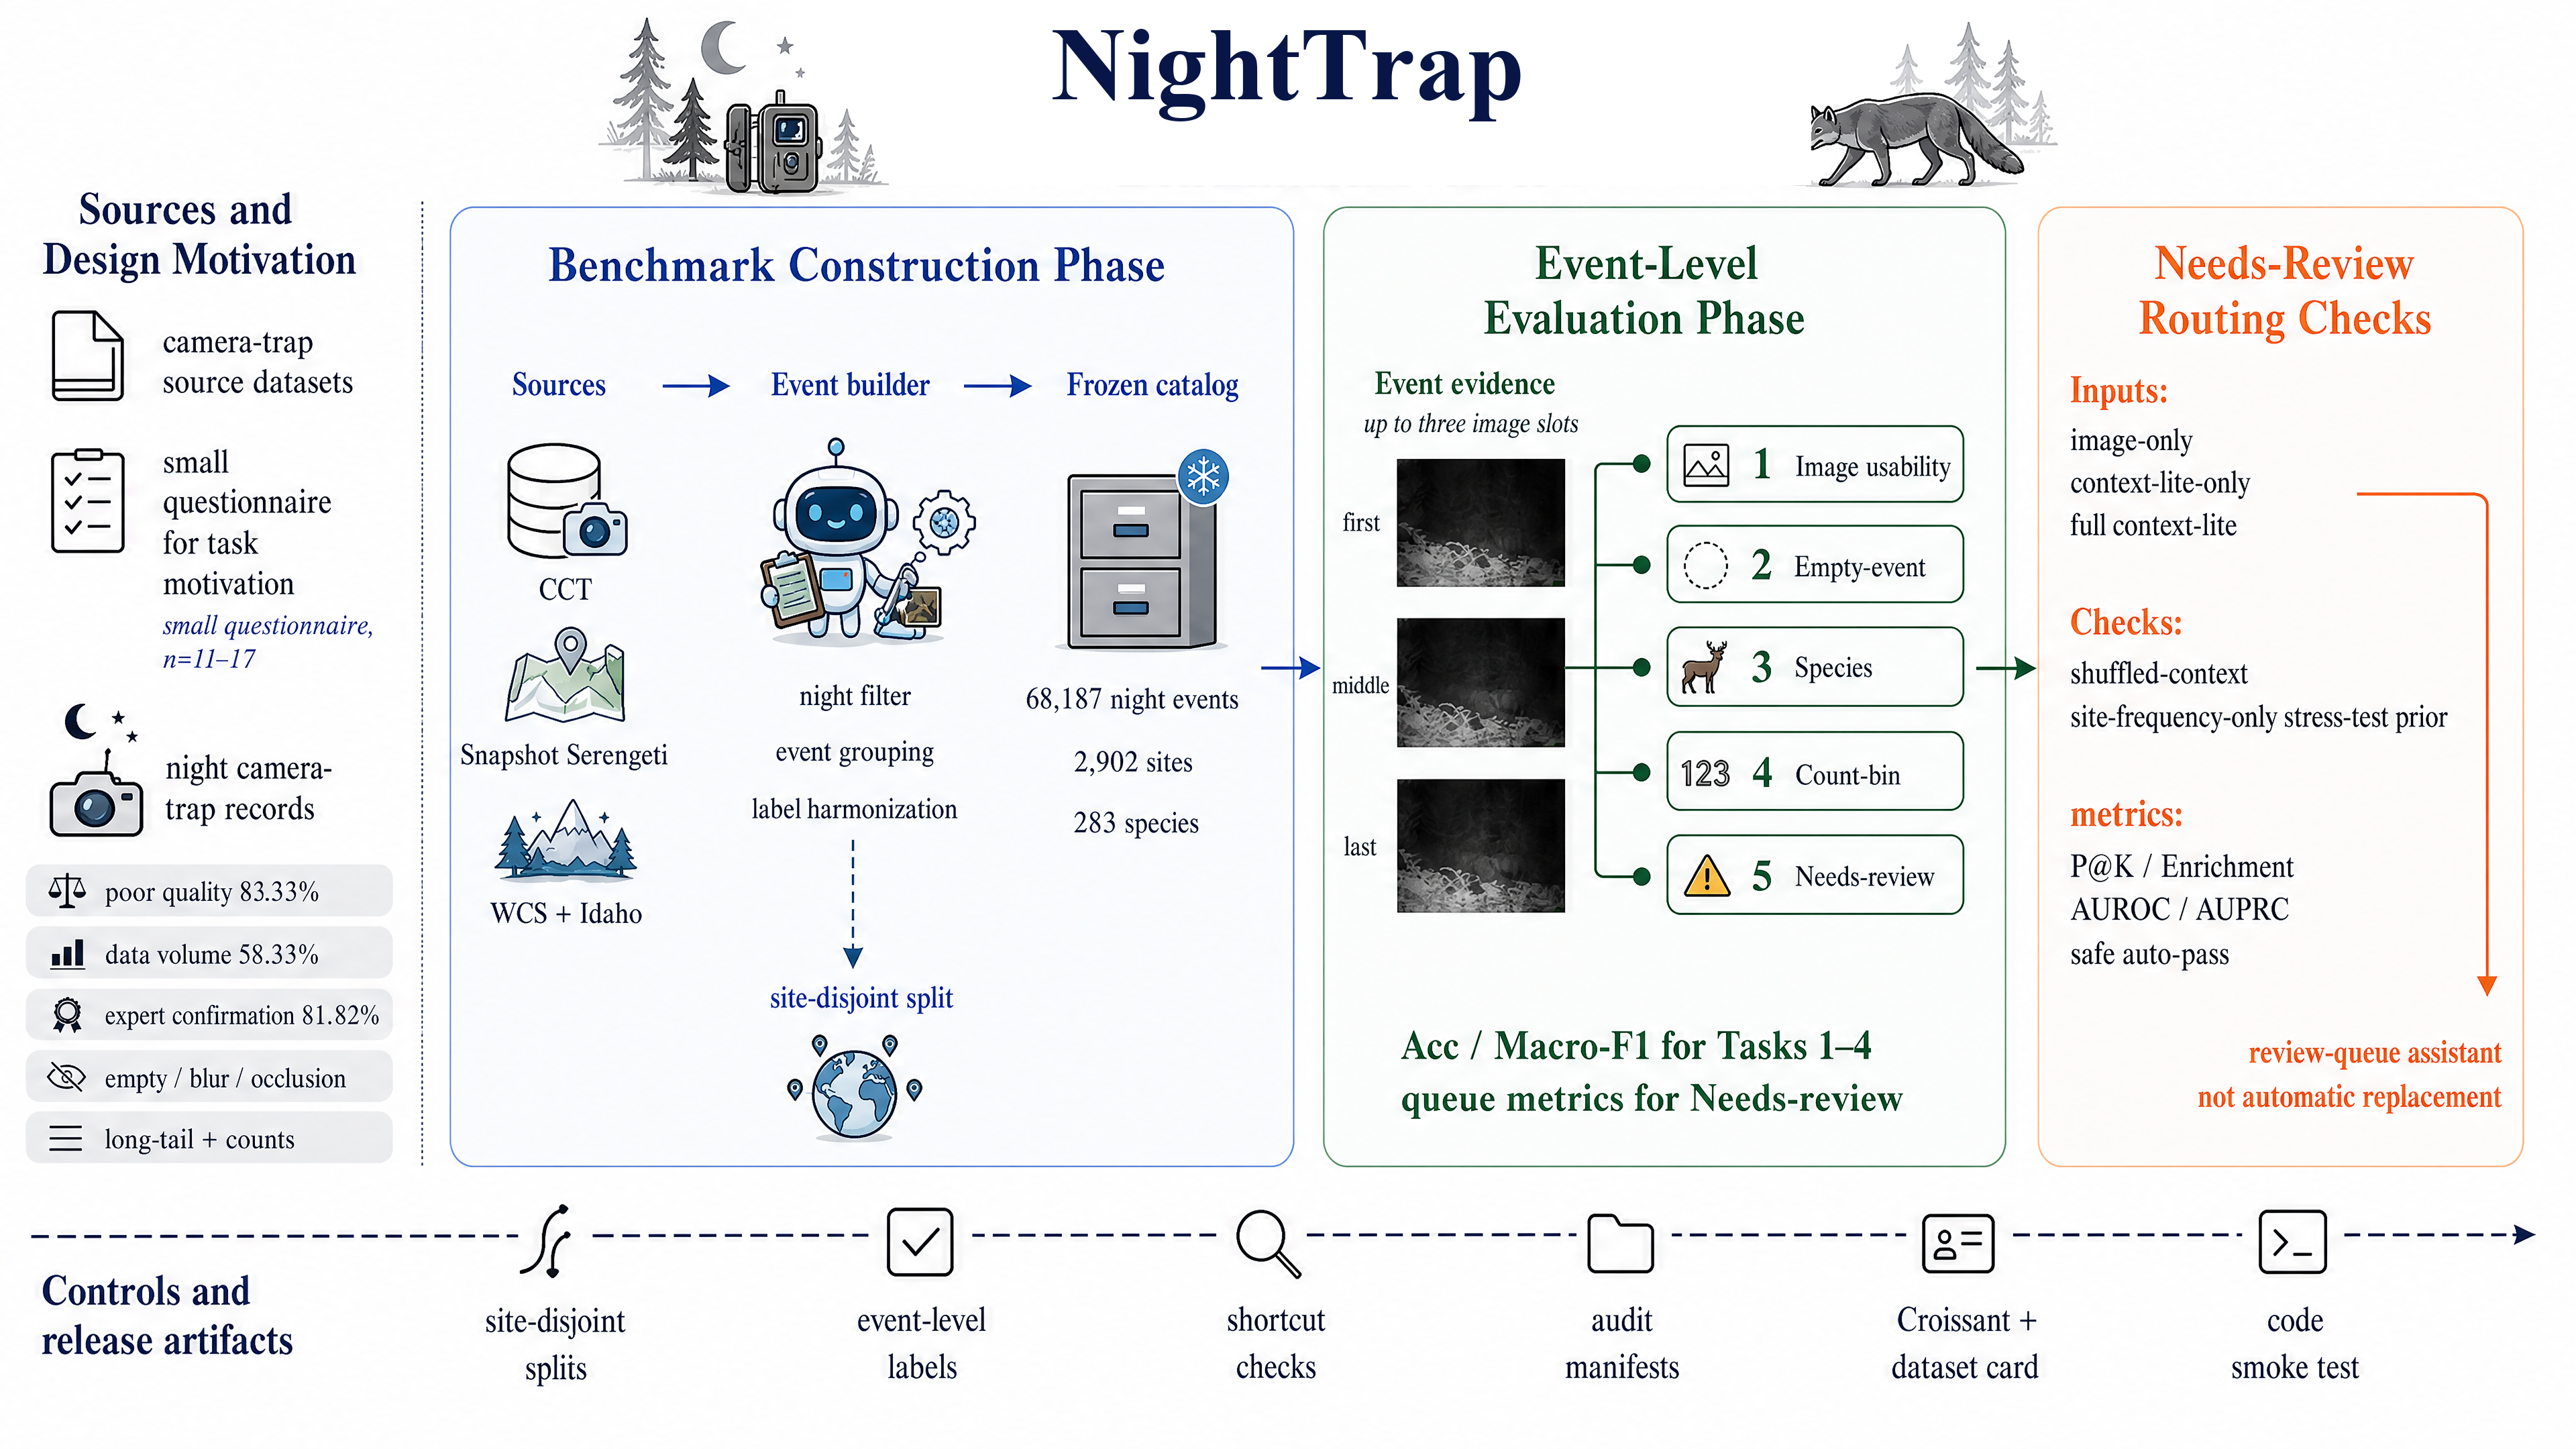
\includegraphics[width=\textwidth]{figures/nighttrap_benchmark_overview_final.png}
\caption{NightTrap benchmark overview. The figure summarizes the design motivation, benchmark construction phase, event-level evaluation phase, and needs-review routing checks. The questionnaire is used only as small-sample task-design motivation; benchmark labels and experimental results are built from the frozen night-event catalog and task-specific construction scripts.}
    \label{fig:nighttrap_benchmark_overview}
\end{figure*}

\subsection{Data construction}

\paragraph{Data sources and frozen event catalog.}
NightTrap is built from four established camera-trap sources: Caltech Camera Traps, Snapshot Serengeti, WCS Camera Traps, and Idaho Camera Traps. We first convert the raw assets into a normalized relational inventory. The inventory contains an event table, a frame table, and lookup tables for source dataset, camera site, species, time, sensor mode, and visibility status. This structure follows dataset-documentation recommendations that emphasize data provenance, intended use, and known limitations \citep{gebru2021datasheets,bender2018datastatements}. It is used only for construction and auditing; models never see database internals. The released benchmark uses a frozen night-event catalog derived from this inventory after night filtering, path validation, event deduplication, and fixed image-slot construction. The final catalog contains \textbf{68,187 night events}, \textbf{115,617 frame records}, \textbf{2,902 camera sites}, and \textbf{283 species}. We define a camera site as the pair of source dataset and source location identifier, because location identifiers are not globally unique across datasets.

\paragraph{Night filtering and event representation.}
We use the catalog field \texttt{time\_of\_day\_bucket = night} to select nocturnal events. Each event keeps up to three fixed image slots: first, middle, and last. This matches how reviewers inspect a trigger burst, but it should not be over-interpreted as uniformly rich temporal evidence. In the frozen catalog, \textbf{64.1\%} of events have identical image paths in all three slots, while \textbf{32.7\%} have three unique image paths. This is why the benchmark evaluates event-level review evidence rather than video understanding.

\paragraph{Task-pool construction.}
Each task is built from the frozen event catalog but uses the most reliable label source for that decision. \textbf{Empty filtering} is built from a MegaDetector-v5a-assisted empty-event asset pool and then rejoined to the frozen catalog. Operationally, detector no-target events define the empty-candidate boundary, while target detections or missing detector status remain \texttt{nonempty\_or\_uncertain}. We use two labels: \texttt{empty\_false\_trigger} and \texttt{nonempty\_or\_uncertain}. The latter intentionally includes uncertain animal cases, because the task is safe empty rejection rather than animal detection at all costs. This detector-assisted construction is a known boundary of the task, so detector rows are treated as screening checks rather than detector-independent proof of true empty-event recognition. \textbf{Species classification} uses closed-set species labels from night events, with dev/test labels required to appear in the training label set. \textbf{Count-bin classification} uses Snapshot Serengeti night events with count labels and maps exact counts into \texttt{1}, \texttt{2}, \texttt{3--5}, and \texttt{6+}; it is therefore a source-constrained count task rather than a claim of cross-source counting coverage. \textbf{Image usability filtering} is a hard evidence-quality set built from candidate examples of sufficient and insufficient visual evidence. \textbf{Needs-review recommendation} is built only from image-usable animal events, so low-quality images are handled upstream rather than being mixed into the human-review decision.

\paragraph{Splits and leakage control.}
All A/B/C task splits are site-disjoint and audited for event, site, and image overlap. Needs-review recommendation uses stricter controls because site context is part of the input. For each target event, the site reference history is built only from earlier events at the same site. The target event itself and future events are excluded. Missing reference history is not backfilled from the full catalog. This prevents the benchmark from turning site context into a hidden answer key.

\begin{table*}[t]
\centering
\caption{NightTrap source and task summary. Panel A summarizes the frozen night-event catalog. Panel B summarizes the five review tasks used in the experiments.}
\label{tab:benchmark_overview}
\small
\setlength{\tabcolsep}{4pt}
\begin{minipage}{0.43\textwidth}
\centering
\textbf{Panel A: source datasets}\par\vspace{0.35em}
\resizebox{\linewidth}{!}{%
\begin{tabular}{lrrr}
\toprule
Dataset & Events & Sites & Species \\
\midrule
Caltech Camera Traps & 24,763 & 136 & 18 \\
Snapshot Serengeti & 22,266 & 212 & 54 \\
WCS Camera Traps & 14,983 & 2,305 & 237 \\
Idaho Camera Traps & 6,175 & 249 & 19 \\
\midrule
Total & 68,187 & 2,902 & 283 \\
\bottomrule
\end{tabular}
}
\end{minipage}
\hfill
\begin{minipage}{0.55\textwidth}
\centering
\textbf{Panel B: review tasks}\par\vspace{0.35em}
\resizebox{\linewidth}{!}{%
\begin{tabular}{lrrrl}
\toprule
Task & Unit & Samples & Sites & Label space \\
\midrule
Image usability & event & 992 & 361 & sufficient / insufficient evidence \\
Empty-event & event & 5,236 & 1,170 & empty false trigger / nonempty-or-uncertain \\
Species & event & 11,837 & 517 & 55 closed-set species \\
Count-bin & event & 22,188 & 212 & 1 / 2 / 3--5 / 6+ \\
Needs-review & event & 6,000 & 480 & routine vs. needs-review \\
\bottomrule
\end{tabular}
}
\end{minipage}
\end{table*}

\subsection{Review workflow tasks}

NightTrap reports five evaluation tasks. Several of these tasks have precedent in prior camera-trap work; our contribution is to place them in one reproducible night review setting and to expose where current models fail under night imaging constraints. The main evidence is task-level, because a single all-in-one score hides whether a model fails at evidence quality, empty filtering, species recognition, counting, or routing. For classification tasks, we use Accuracy as the overall fraction of correct predictions and macro-averaged F1 (Macro-F1) to measure performance under class imbalance, because each class contributes equally regardless of frequency.

\begin{figure}[t]
\centering
\includegraphics[width=0.95\linewidth]{figures/nighttrap_review_task_map.png}
\caption{NightTrap review-task map. The benchmark organizes night camera-trap review into five decision points and reports task-level metrics rather than an unattended cascade score. Task 5 additionally separates Visual Only, Context Only, Combined, and Shortcut Check settings to test context-shortcut risk.}
\label{fig:review_task_map}
\end{figure}

\paragraph{Task definitions.}
\textbf{Image usability filtering} asks whether visual evidence is sufficient for downstream review. It is not an animal-presence task: a usable image may be empty, and an unusable image may still contain an animal that is too dark, blurred, occluded, or overexposed. \textbf{Empty-event filtering} asks whether an event is a safe empty trigger. We use \texttt{empty\_false\_trigger} versus \texttt{nonempty\_or\_uncertain} from a MegaDetector-v5a-assisted pool matched back to the frozen night catalog; ambiguous animal-like cases stay conservative, so detector rows are construction-boundary checks rather than detector-independent ceilings. \textbf{Species classification} is closed-set recognition over 55 night-event species with site-disjoint splits. \textbf{Count-bin classification} uses Snapshot Serengeti night events and maps counts to \texttt{1}, \texttt{2}, \texttt{3--5}, and \texttt{6+}; it is source-constrained rather than cross-source counting coverage. \textbf{Needs-review recommendation} asks whether an image-usable animal event should enter the human review queue. \texttt{routine} maps to \texttt{needs\_review}=0 and \texttt{review} to \texttt{needs\_review}=1. These labels are a fixed review-routing rule, not universal ecological truth or expert consensus. Classification tasks report Accuracy and Macro-F1; Task 5 additionally reports P@K, Enrichment@K, AUROC/AUPRC where available, NDCG, and high-recall safe auto-pass.

\begin{figure}[t]
\centering
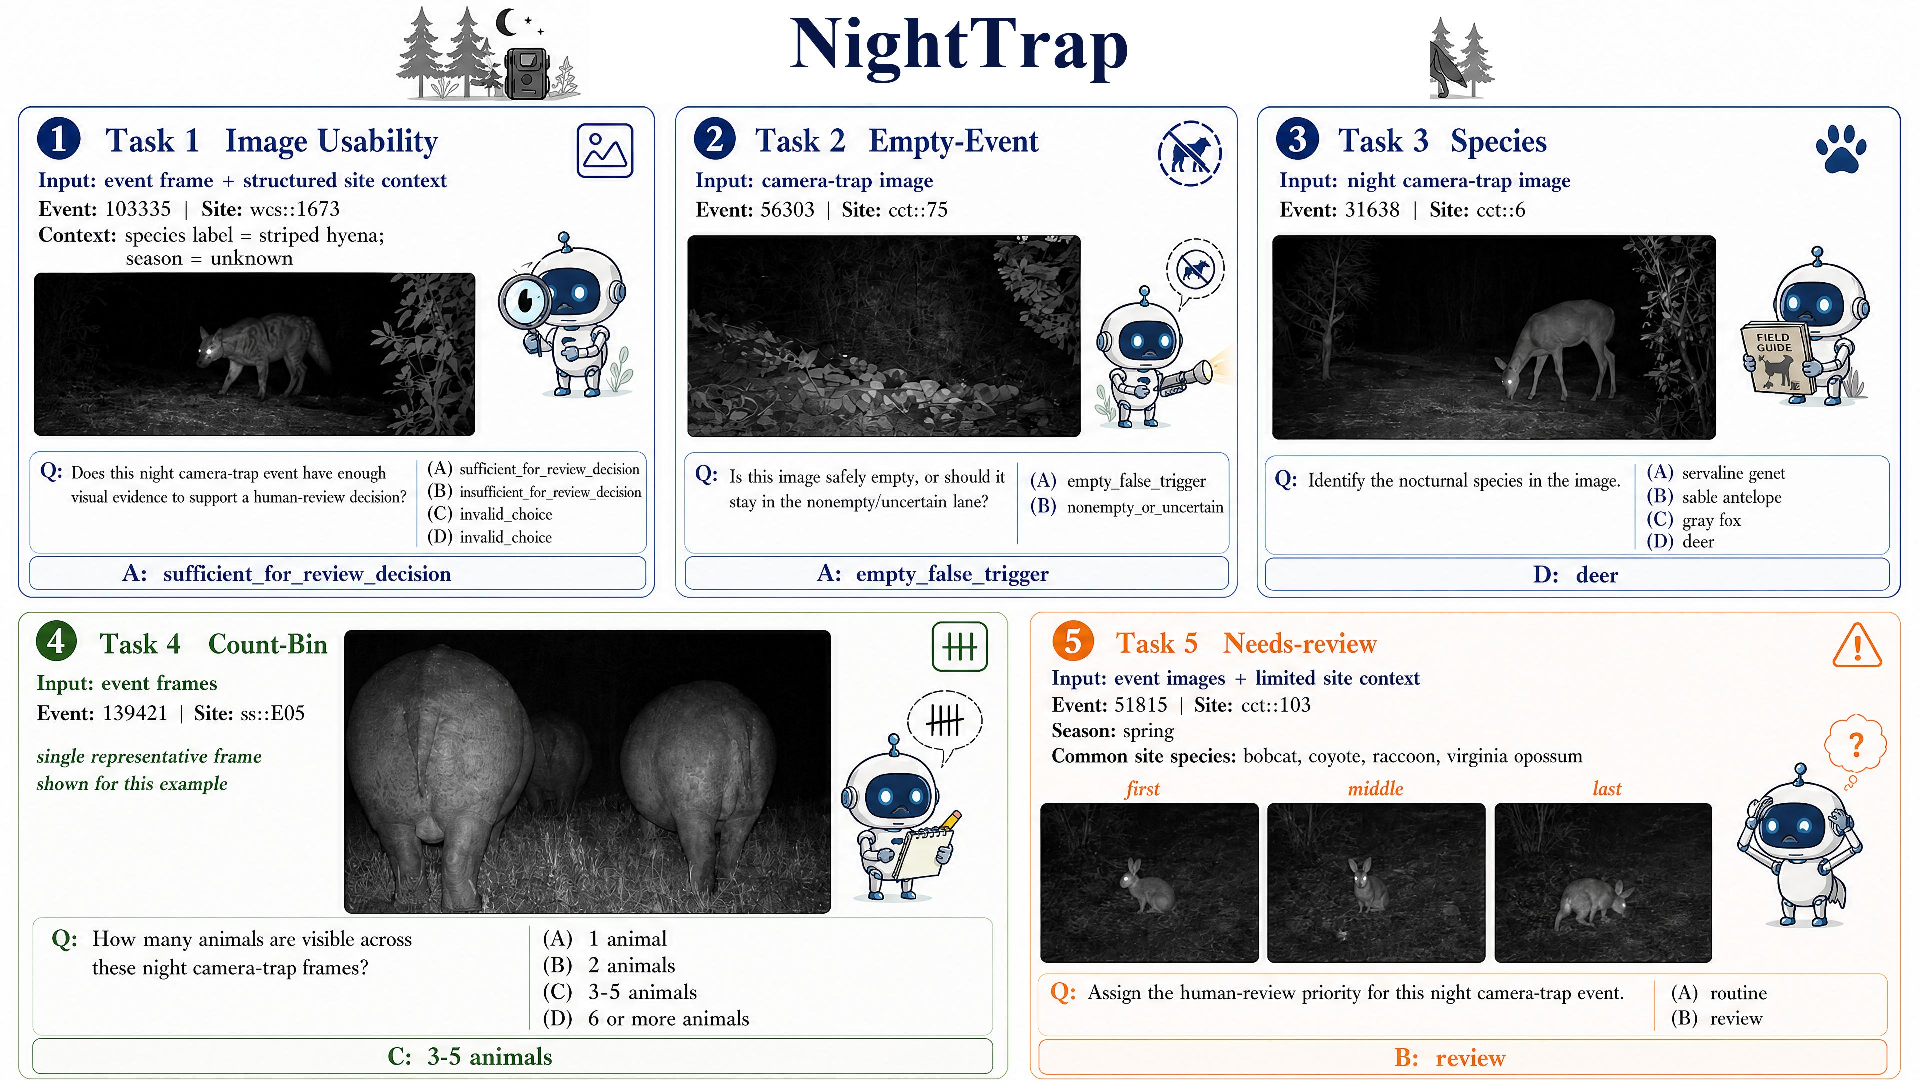
\includegraphics[width=0.95\linewidth]{figures/nighttrap_qa_examples_final.pdf}
\caption{Representative NightTrap QA examples across the five review tasks. Each card shows the released question format, answer choices, and target answer for one decision point; Task 5 uses binary routine-versus-review output plus continuous review scores for queue ordering.}
\label{fig:qa_examples}
\end{figure}

\paragraph{Task 5 input settings and sets.}
For needs-review recommendation, NightTrap simulates lightweight reviewer knowledge while excluding answer-revealing fields such as the current species label, novelty flag, rarity label, future events, or the gold decision. We use four controlled input views: \textbf{Visual Only}, \textbf{Context Only}, \textbf{Combined}, and \textbf{Shortcut Checks} with perturbed or reduced context. These are input settings, not different tasks.

NightTrap uses four needs-review sets for different purposes. The \textbf{Main Queue Set} ($N=6000$) is the main queue benchmark with a 30\% needs-review base rate. The \textbf{Input Stress-Test} ($N=983$) is review-heavy, with 85.8\% positives after binary collapse, so it is not a deployment base-rate estimate. The \textbf{Ranker Sub-split} ($N=913$) is the frozen supervised-ranker subset with available CLIP embeddings and valid context features. The \textbf{Diagnostic Cascade} ($N=150$) is an all-in-one smoke check. These sets answer different questions and are not interchangeable leaderboards.

\subsection{Distribution and annotation reliability}

NightTrap preserves source heterogeneity: datasets differ in site density, species composition, geography, label granularity, and night imaging mode. Species and sites are long-tailed, with a median of 12 night events per species and 5 night events per site, so we report Macro-F1, per-task checks, and ranking metrics rather than only accuracy.

For image usability, a paired audit gives 72.5\% three-way usable/unusable/uncertain agreement with Cohen's $\kappa=0.441$ across 298 valid annotations. The operational decision is binary: whether evidence can be trusted for downstream review. Excluding uncertain cases yields 98.5\% agreement with $\kappa=0.911$, and grouping uncertain with unsafe or boundary evidence yields 86.9\% agreement with $\kappa=0.703$.

For needs-review, we do not claim that \texttt{review} is an expert ecological-review label. In a 100-event matched-context model-assisted audit, 98 rows were binary-evaluable and 2 were uncertain. Agreement with the benchmark rule was 64.3\% with Cohen's $\kappa=0.286$. This is a plausibility check, not a multi-expert agreement study, and it reinforces that needs-review should be judged by queue enrichment and safe auto-pass behavior.




\section{Experiments and Results}
\label{sec:experiments_results}

\subsection{Experimental setup}

\paragraph{Evaluation metrics.}
NightTrap evaluates four review-workflow classification tasks and one human-review recommendation task. Image usability, Empty-event, Species, and Count-bin report Accuracy and Macro-F1, with Macro-F1 as the primary metric because night camera-trap labels are imbalanced and long-tailed \citep{lin2017focalloss,gupta2019lvis}. Needs-review recommendation is evaluated by the operational question each metric answers:
\textbf{Binary decision} metrics test whether a model follows the fixed routine-versus-review rule. \textbf{Queue ordering} metrics test whether needs-review events appear near the top of a limited review queue: P@K reports top-queue precision, Enrichment@K divides P@K by the positive base rate, AUROC and AUPRC summarize threshold-independent binary scores under class imbalance \citep{davis2006prroc}, and NDCG is retained as a secondary graded-ranking check where continuous review scores are frozen \citep{jarvelin2002ndcg}. \textbf{Workload reduction} is measured by safe auto-pass: for a target needs-review recall $r$, it reports the largest fraction of events that can be automatically passed while maintaining recall at least $r$, following the selective-prediction principle that abstention and automation require their own operating analysis \citep{geifman2017selective}. These metrics are grouped by review use case rather than treated as one interchangeable score list. Selected bootstrap intervals for the main classification rows and needs-review queue metrics are reported in Appendix Tables~\ref{tab:main_classification_ci} and~\ref{tab:task5_bootstrap_ci}.

\paragraph{Models.}
We group evaluated models by their role in the review workflow. Naive baselines include majority-class prediction, random scoring, and rule-only checks. Supervised vision baselines include CLIP and DINOv2 probes, ViT-B/16 and ConvNeXt-Tiny fine-tunes, detector-crop species baselines, and MegaDetector-assisted empty screening. VLM baselines include Qwen2-VL-2B and Qwen3-VL-8B without NightTrap-specific fine-tuning; GPT rows are retained only as closed-source exploratory references. Task-5 rankers include CLIP+Context logistic rankers, XGBoost~\citep{chen2016xgboost}, and LightGBM~\citep{ke2017lightgbm} variants. Full commands and run details are reported in the appendix.

\subsection{Performance across question types}

In Table~\ref{tab:workflow_main}, we compare representative model performance across the four NightTrap classification tasks. Closed-source, open-source, and conventional camera-trap baselines are shown separately so that capability comparisons do not mix reproducibility status with raw score differences.

\begin{table}[t]
\centering
\caption{Representative classification results. Values are Macro-F1 percentages; Accuracy is reported in the full appendix tables.}
\label{tab:workflow_main}
\small
\begin{tabular}{lrrrr}
\toprule
Model & Usability & Empty & Species & Count-bin \\
\midrule
GPT-5.4 reference & 79.04 & 81.68 & 34.13 & 64.48 \\
Qwen2-VL-2B & 34.63 & 62.88 & 29.87 & 42.29 \\
Qwen3-VL-8B & \textbf{83.64} & 75.24 & \textbf{48.09} & 58.66 \\
CLIP linear probe & 68.20 & 75.25 & 35.58 & 49.06 \\
Best supervised vision baseline & 81.78 & \textbf{80.13} & 39.50 & \textbf{59.70} \\
\bottomrule
\end{tabular}
\end{table}

\FloatBarrier

The per-task best row is not a single model; full supervised rows are in the appendix. The first pattern is that easier-looking screening decisions are still not solved uniformly. Qwen3-VL-8B reaches the best open-source score on image usability, but the same model remains well below perfect on empty filtering. We therefore treat detector-assisted empty-pool construction as screening infrastructure rather than as detector-independent evidence that the empty-event task is solved. The second pattern is that species recognition remains the largest classification gap: Qwen3-VL-8B has high species Accuracy but much lower Macro-F1, indicating uneven behavior across long-tailed and ambiguous taxa. The species interface also differs by model family: VLM rows answer the released four-choice species question, whereas supervised vision rows are closed-set classifiers over the species label set. We therefore avoid treating the VLM species row as a closed-set supervised ceiling; Appendix Table~\ref{tab:species_candidate_alignment} adds a candidate-set alignment diagnostic. Count-bin classification is also difficult because multiple animals, overlapping bodies, and partial visibility turn simple recognition into event-level reasoning.

A longer ConvNeXt-Tiny species convergence check improves the 2-epoch fine-tune from 21.34 to 36.75 Macro-F1, confirming that the initial short fine-tune underestimates what task-specific supervised training can do. This does not change the main best-supervised species row, because the DINOv2 full-frame linear probe remains higher at 39.50 Macro-F1, but it changes the interpretation: NightTrap should not be read as showing a blanket VLM advantage over supervised vision baselines. The stronger conclusion is narrower: current VLMs are competitive on some review decisions, while long-tail species Macro-F1 remains difficult for both VLM and supervised baselines.

Table~\ref{tab:needs_review_main} reports Task 5 separately, and Figure~\ref{fig:task5_core_performance} visualizes the main queue metrics. The Main Queue Set is the realistic routine-heavy setting. Ranker rows use the frozen Ranker Sub-split because the CLIP scripts require available image embeddings and valid context features. Clean tree-ranker rows exclude audit flags, audit-only current-species support fields, and site common-species name expansion. The Input Stress-Test remains an input and queue-ordering diagnostic, not the primary fifth task.

\begin{table}[t]
\centering
\caption{Representative needs-review results. These rows answer different questions and should not be read as one leaderboard.}
\label{tab:needs_review_main}
\small
\begin{tabular}{llrrrr}
\toprule
Split & Model / input & Base & P@50 & Enrich@50 & Auto-pass@95R \\
\midrule
Main Queue & Qwen3-VL-8B, Combined & 30.00 & 66.00 & 2.20$\times$ & 7.42 \\
Ranker Sub-split & XGBoost Visual Only & 25.30 & 56.00 & 2.21$\times$ & 3.40 \\
Ranker Sub-split & LightGBM Visual Only & 25.30 & 54.00 & 2.13$\times$ & 4.27 \\
Ranker Sub-split & CLIP+Context logistic & 25.30 & 32.00 & 1.26$\times$ & 8.43 \\
Input Stress-Test & Qwen3-VL-8B, Combined & 85.76 & 66.00 & 0.77$\times$ & n/a \\
Input Stress-Test & NVILA-8B, Combined & 85.76 & 78.00 & 0.91$\times$ & n/a \\
\bottomrule
\end{tabular}
\end{table}

\FloatBarrier

\begin{figure}[!htbp]
\centering
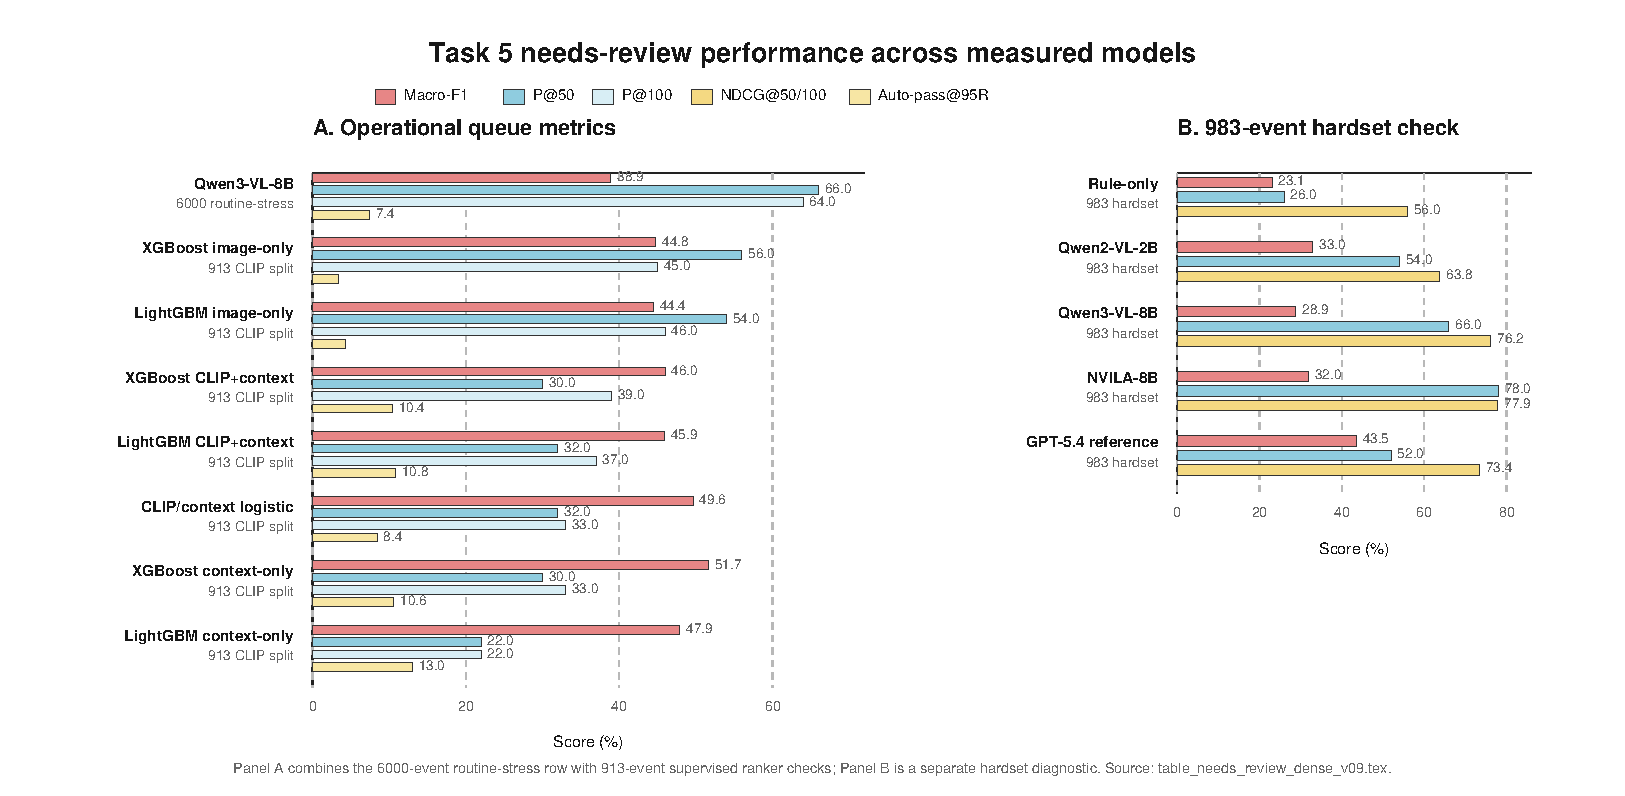
\includegraphics[width=0.95\linewidth]{figures/nighttrap_task5_core_performance.pdf}
\caption{Core Task 5 needs-review performance. Panel A summarizes operational queue metrics for the Main Queue Set and Ranker Sub-split checks; Panel B shows the Input Stress-Test diagnostic with its high P@50 base-rate reference.}
\label{fig:task5_core_performance}
\end{figure}

\FloatBarrier

On the Main Queue Set, Qwen3-VL-8B reaches P@50 of 66.00 at a 30.00 base rate, a 2.20$\times$ enrichment over random ranking. Its needs-review score also gives AUROC 57.88 and AUPRC 38.44, while the P@50 bootstrap interval remains wide at [54.00, 78.00]. This is useful for queue ordering, but not the same as safe workload reduction: at 95\% needs-review recall, Qwen3-VL-8B automatically passes only 7.42\% of events, and at 98\% recall this falls to 3.35\%. The CLIP+Context logistic ranker passes 8.43\% and 4.27\% at the same recall targets on the Ranker Sub-split. Current models therefore help decide what humans should see first more than what humans never need to see, which is the intended distinction between review prioritization and automatic exclusion.

We also ran a 150-event all-in-one smoke check in which Qwen3-VL-8B had to output evidence quality, empty status, species, count bin, review decision, and a review score. After collapsing \texttt{review} and \texttt{priority\_review} into binary \texttt{needs\_review}, the model reaches 42.67\% Accuracy, 39.93\% Macro-F1, 54.11 AUROC, 64.87 AUPRC, and only 16.84\% needs-review recall; P@50 is 72.00\% at a 63.33\% base rate, or 1.14$\times$ enrichment. This diagnostic supports decision-point reporting because a single all-in-one score hides whether failure comes from visual evidence, empty filtering, species, count, or review routing. Full numbers are in Appendix~\ref{tab:end2end_smoke}.

\subsection{Ablations and shortcut checks}

Appendix Table~\ref{tab:ablation_diagnostics} condenses the ablations and shortcut checks. On the Ranker Sub-split, shuffled context reaches P@50 of 36.00 while the matched CLIP+Context logistic row reaches 32.00, and a site-frequency-only stress prior reaches P@50 of 64.00. We therefore treat site history as useful reviewer-side information with shortcut risk, not stable evidence of visual grounding. In practice, this means that context-aware models should be reported alongside visual-only and perturbed-context controls before they are used to route scarce expert attention. The remaining checks show that more image slots do not automatically help, night-IR changes needs-review behavior, count-bin evaluation is source-constrained, and the empty pool remains detector-assisted.

\section{Conclusion}

% NightTrap 评估夜间相机陷阱审核流程，包括五个任务：Image usability filtering、Empty-event filtering、Species classification、Count-bin classification 和 Needs-review recommendation。它将不可判读图像与空图分开，并且只在图像可判读的动物事件上评估人工审核推荐。
NightTrap evaluates night camera-trap triage around species recognition: models judge usable evidence, filter empty events, classify species, estimate count bins, and prioritize image-usable animal events for human review. Its contribution is not a new species taxonomy or an unconstrained ecological reasoning task, but a workflow-structured benchmark that separates recognition, queue enrichment, and recall-constrained safe pass-through. Current VLMs can help order queues, but safe automatic pass-through remains small at high needs-review recall, and species accuracy can hide long-tail failures behind much lower Macro-F1. Site history is informative but shortcut-prone: in lightweight rankers, context can reduce early queue precision or underperform shuffled context, so context-aware review models need Visual Only, Context Only, Combined, and Shortcut Check settings. The all-in-one smoke check further shows why unattended full automation is unsafe. For deployment-oriented evaluation, the practical lesson is that camera-trap assistance should be reported as a set of operating points: what can be hidden, what should be surfaced early, and which failures remain visible to human reviewers. NightTrap makes these distinctions explicit so future systems can improve workflow value without turning a review-routing benchmark into an unsupported automation claim.

\paragraph{Limitations and future work.}
The needs-review label is a review-routing label rather than expert ecological ground truth; the matched-context audit is model-assisted and single-annotator rather than a multi-expert agreement study \citep{northcutt2021labelerrors}. The Main Queue Set is the main queue benchmark, while the Input Stress-Test is a review-heavy input check. Count-bin evaluation is source-constrained, the empty-event set inherits risk from MegaDetector-assisted pool construction, and frozen VLM choice scores should not be read as calibrated deployment probabilities \citep{guo2017calibration}. NightTrap focuses on night events and does not yet cover daytime review, behavior annotation, open-ended ecological reporting, or causal reasoning. Because source datasets differ in camera placement, species vocabulary, and annotation conventions, benchmark results should also be interpreted as evidence about this normalized review workflow rather than as direct estimates of population abundance or ecological trend quality. The current tasks likewise evaluate event-level review decisions, not downstream ecological inference such as occupancy modeling, abundance estimation, or intervention planning. The present release evaluates fixed prompts and frozen model snapshots rather than adaptive review interfaces, so it should be read as a reproducible benchmark layer below any field deployment study. Future versions should add independent expert audits, external camera-site validation, stronger license and provenance reporting for upstream assets, and daytime/night transfer checks before treating review-routing scores as deployment-ready evidence.

\clearpage
\begingroup
\footnotesize
\begin{thebibliography}{99}

\bibitem{norouzzadeh2017snapshot}
M. S. Norouzzadeh, A. Nguyen, M. Kosmala, A. Swanson, M. Palmer, C. Packer, and J. Clune.
Automatically Identifying, Counting, and Describing Wild Animals in Camera-Trap Images with Deep Learning.
\emph{Proceedings of the National Academy of Sciences}, 115(25):E5716--E5725, 2018.

\bibitem{schneider2018camera}
S. Schneider, G. W. Taylor, and S. C. Kremer.
Deep Learning Object Detection Methods for Ecological Camera Trap Data.
\emph{2018 15th Conference on Computer and Robot Vision (CRV)}, pp. 321--328, 2018.
doi:10.1109/CRV.2018.00052.

\bibitem{choinski2021first}
M. Choi{\'n}ski, M. Rogowski, P. Tynecki, D. P. J. Kuijper, M. Churski, and J. W. Bubnicki.
A First Step Towards Automated Species Recognition from Camera Trap Images of Mammals Using AI in a European Temperate Forest.
In \emph{Computer Information Systems and Industrial Management (CISIM 2021)}, Lecture Notes in Computer Science 12883, pp. 299--310. Springer, 2021.
doi:10.1007/978-3-030-84340-3\_24.

\bibitem{beery2019iwildcam}
S. Beery, D. Morris, and P. Perona.
The iWildCam 2019 Challenge Dataset.
\emph{arXiv preprint arXiv:1907.07617}, 2019.

\bibitem{koh2021wilds}
P. W. Koh et al.
WILDS: A Benchmark of in-the-Wild Distribution Shifts.
\emph{Proceedings of the International Conference on Machine Learning}, 2021.

\bibitem{gomez2016towards}
A. Gomez Villa, A. Salazar, and F. Vargas.
Towards Automatic Wild Animal Monitoring: Identification of Animal Species in Camera-trap Images Using Very Deep Convolutional Neural Networks.
\emph{Ecological Informatics}, 41:24--32, 2017.
doi:10.1016/j.ecoinf.2017.07.004.

\bibitem{beery2019pipeline}
S. Beery, D. Morris, and S. Yang.
Efficient Pipeline for Camera Trap Image Review.
\emph{arXiv preprint arXiv:1907.06772}, 2019.

\bibitem{radford2021clip}
A. Radford, J. W. Kim, C. Hallacy, A. Ramesh, G. Goh, S. Agarwal, G. Sastry, A. Askell, P. Mishkin, J. Clark, G. Krueger, and I. Sutskever.
Learning Transferable Visual Models From Natural Language Supervision.
\emph{Proceedings of the International Conference on Machine Learning}, 2021.

\bibitem{oquab2023dinov2}
M. Oquab et al.
DINOv2: Learning Robust Visual Features without Supervision.
\emph{Transactions on Machine Learning Research}, 2024.

\bibitem{dosovitskiy2021vit}
A. Dosovitskiy et al.
An Image is Worth 16x16 Words: Transformers for Image Recognition at Scale.
\emph{Proceedings of the International Conference on Learning Representations}, 2021.

\bibitem{liu2022convnext}
Z. Liu, H. Mao, C.-Y. Wu, C. Feichtenhofer, T. Darrell, and S. Xie.
A ConvNet for the 2020s.
\emph{Proceedings of the IEEE Conference on Computer Vision and Pattern Recognition}, 2022.

\bibitem{gupta2019lvis}
A. Gupta, P. Dollar, and R. Girshick.
LVIS: A Dataset for Large Vocabulary Instance Segmentation.
\emph{Proceedings of the IEEE Conference on Computer Vision and Pattern Recognition}, 2019.

\bibitem{vanhorn2018inaturalist}
G. Van Horn et al.
The iNaturalist Species Classification and Detection Dataset.
\emph{Proceedings of the IEEE Conference on Computer Vision and Pattern Recognition}, 2018.

\bibitem{lin2017focalloss}
T.-Y. Lin, P. Goyal, R. Girshick, K. He, and P. Dollar.
Focal Loss for Dense Object Detection.
\emph{Proceedings of the IEEE International Conference on Computer Vision}, 2017.

\bibitem{fabian2023wildmatch}
Z. Fabian et al.
Multimodal Foundation Models for Zero-shot Animal Species Recognition in Camera Trap Images.
\emph{arXiv preprint arXiv:2311.01064}, 2023.

\bibitem{jing2024animalbench}
Y. Jing, R. Zhang, K. Liang, Y. Li, Z. He, Z. Ma, and J. Guo.
Animal-Bench: Benchmarking Multimodal Video Models for Animal-centric Video Understanding.
\emph{Advances in Neural Information Processing Systems}, 2024.

\bibitem{ng2022animalkingdom}
X. L. Ng, K. E. Ong, Q. Zheng, Y. Ni, S. Y. Yeo, and J. Liu.
Animal Kingdom: A Large and Diverse Dataset for Animal Behavior Understanding.
\emph{Proceedings of the IEEE Conference on Computer Vision and Pattern Recognition}, 2022.

\bibitem{chen2023mammalnet}
J. Chen, M. Hu, D. J. Coker, M. L. Berumen, B. Costelloe, S. Beery, A. Rohrbach, and M. Elhoseiny.
MammalNet: A Large-scale Video Benchmark for Mammal Recognition and Behavior Understanding.
\emph{Proceedings of the IEEE Conference on Computer Vision and Pattern Recognition}, 2023.

\bibitem{vyskocil2024zeroshot}
J. Vysko{\v{c}}il and L. Picek.
Towards Zero-Shot Camera Trap Image Categorization.
In \emph{Computer Vision -- ECCV 2024 Workshops}, pp. 37--53. Springer, 2024.
doi:10.1007/978-3-031-92387-6\_3.

\bibitem{alayrac2022flamingo}
J.-B. Alayrac et al.
Flamingo: A Visual Language Model for Few-Shot Learning.
\emph{Advances in Neural Information Processing Systems}, 2022.

\bibitem{li2023blip2}
J. Li, D. Li, S. Savarese, and S. Hoi.
BLIP-2: Bootstrapping Language-Image Pre-training with Frozen Image Encoders and Large Language Models.
\emph{Proceedings of the International Conference on Machine Learning}, 2023.

\bibitem{gebru2021datasheets}
T. Gebru et al.
Datasheets for Datasets.
\emph{Communications of the ACM}, 2021.

\bibitem{bender2018datastatements}
E. M. Bender and B. Friedman.
Data Statements for Natural Language Processing: Toward Mitigating System Bias and Enabling Better Science.
\emph{Transactions of the Association for Computational Linguistics}, 2018.

\bibitem{mitchell2019modelcards}
M. Mitchell et al.
Model Cards for Model Reporting.
\emph{Proceedings of the Conference on Fairness, Accountability, and Transparency}, 2019.

\bibitem{jarvelin2002ndcg}
K. Jarvelin and J. Kekalainen.
Cumulated Gain-Based Evaluation of IR Techniques.
\emph{ACM Transactions on Information Systems}, 2002.

\bibitem{davis2006prroc}
J. Davis and M. Goadrich.
The Relationship Between Precision-Recall and ROC Curves.
\emph{Proceedings of the International Conference on Machine Learning}, 2006.

\bibitem{geifman2017selective}
Y. Geifman and R. El-Yaniv.
Selective Classification for Deep Neural Networks.
\emph{Advances in Neural Information Processing Systems}, 2017.

\bibitem{chen2016xgboost}
T. Chen and C. Guestrin.
XGBoost: A Scalable Tree Boosting System.
\emph{Proceedings of the ACM SIGKDD Conference on Knowledge Discovery and Data Mining}, 2016.

\bibitem{ke2017lightgbm}
G. Ke et al.
LightGBM: A Highly Efficient Gradient Boosting Decision Tree.
\emph{Advances in Neural Information Processing Systems}, 2017.

\bibitem{northcutt2021labelerrors}
C. G. Northcutt, A. Athalye, and J. Mueller.
Pervasive Label Errors in Test Sets Destabilize Machine Learning Benchmarks.
\emph{Advances in Neural Information Processing Systems}, 2021.

\bibitem{guo2017calibration}
C. Guo, G. Pleiss, Y. Sun, and K. Q. Weinberger.
On Calibration of Modern Neural Networks.
\emph{Proceedings of the International Conference on Machine Learning}, 2017.

\end{thebibliography}
\endgroup

\clearpage
\appendix

\section{Appendix Overview}

\begin{appendixbox}[title={What the appendix contains}]{NightTrapBlue}
The appendix is organized around reproducibility and review use. Appendix~\ref{app:release_reproducibility} documents the release package, data-access constraints, result inventory, compute notes, LLM/VLM usage, broader impacts, and questionnaire notes. Appendix~\ref{app:questionnaire_instrument} gives the translated questionnaire instrument used only to motivate task design. Appendix~\ref{app:additional_tables} provides the full check tables and run details behind the compact main-text results.
\end{appendixbox}

\begin{appendixbox}[title={How to read the needs-review tables}]{NightTrapGold}
The appendix keeps the needs-review sample counts separate. The Main Queue Set ($N=6000$) is the main operational queue with a 30\% needs-review base rate. The Input Stress-Test ($N=983$) is a controlled, review-heavy input-setting check. The Ranker Sub-split ($N=913$) is a supervised-ranker check retained after requiring frozen CLIP embeddings and valid context features. The Diagnostic Cascade ($N=150$) is an all-in-one smoke check. These sets answer different questions and should not be merged into a single leaderboard.
\end{appendixbox}

\section{Artifact, Release, and Reproducibility}
\label{app:release_reproducibility}

NightTrap is a derived benchmark over existing camera-trap sources. The release provides benchmark metadata, task splits, labels, prompts, evaluation artifacts, Croissant metadata, and code under CC BY-NC 4.0 for the derived NightTrap assets, but it does not redistribute raw images whose source datasets impose independent access or license terms. Users obtain raw images from the original data providers and use the released metadata and scripts to rebuild benchmark views. The anonymous dataset repository is \url{https://huggingface.co/datasets/LohseRre/nighttrap-eandd2026}, and the anonymous code repository is \url{https://github.com/LohseZSai/nighttrap_eandd2026}. The release boundary is therefore derived benchmark assets only: raw images and model weights remain governed by their upstream provider terms.

\begin{table*}[h]
\centering
\caption{Release package. ``Restricted'' and ``not redistributed'' entries are included to avoid promising release rights that depend on upstream source datasets.}
\label{tab:release_package}
\scriptsize
\setlength{\tabcolsep}{3pt}
\begin{tabularx}{\textwidth}{p{3.0cm}p{2.4cm}X}
\toprule
Artifact & Release status & Notes \\
\midrule
Frozen event catalog & anonymized & Event IDs, source keys, site keys, metadata, image-slot paths, and audit fields with sensitive location fields removed or coarsened. \\
Task split files & released & Train/dev/test splits and label files for Image usability, Empty-event, Species, Count-bin, and Needs-review tasks. \\
Context-lite construction code & released & Builds prior site-history context from earlier same-site events only; excludes current and future events. \\
Evaluation scripts & released & Metric scripts for classification, ranking, enrichment, safe auto-pass, and appendix checks. \\
Baseline scripts & released & CLIP linear probe, MegaDetector threshold, CLIP+Context ranker, and check scripts used for reported tables. \\
Code repository & available & Anonymous GitHub repository with release smoke test, requirements, paper source snapshot, and reproducibility scripts that do not include raw images or local paths. \\
Prompt templates & released & Fixed VLM prompts and answer schemas used for Qwen and reference VLM evaluations. \\
Metadata schema & released & Field definitions for event catalog, task rows, labels, allowed context fields, and prediction files. \\
Dataset card & released & Documents scope, intended use, label construction, limitations, and known biases in the anonymous Hugging Face dataset repository. \\
Croissant file & validated & Machine-readable metadata includes the required NeurIPS RAI fields and points to the dataset repository, code repository, and upstream raw-image access instructions. \\
Raw images & not redistributed & Raw images remain governed by original source dataset terms; users must obtain them from Caltech Camera Traps, Snapshot Serengeti, WCS Camera Traps, and Idaho Camera Traps as allowed. \\
\bottomrule
\end{tabularx}
\end{table*}

\begin{table*}[h]
\centering
\caption{License and data-access inventory. NightTrap releases derived metadata, labels, splits, prompts, and code; raw images are not redistributed and remain governed by upstream provider terms.}
\label{tab:license_data_access}
\scriptsize
\setlength{\tabcolsep}{2.5pt}
\begin{tabularx}{\textwidth}{p{2.25cm}p{2.4cm}p{2.45cm}p{2.0cm}X p{2.45cm}}
\toprule
Asset & Source & License or terms & Redistribution? & Used fields or outputs & Citation / URL \\
\midrule
Caltech Camera Traps & Original CCT dataset & upstream terms apply & raw images not redistributed & Images are referenced through derived metadata; species/site/time fields are used for benchmark construction & \citep{beery2019iwildcam}; original provider access required \\
Snapshot Serengeti & Snapshot Serengeti dataset & upstream terms apply & raw images not redistributed & Species labels, count labels, timestamps, and image references & \citep{norouzzadeh2017snapshot}; original provider access required \\
WCS Camera Traps & WCS source & upstream terms apply & raw images not redistributed & Species labels, site keys, timestamps, and image references & \href{https://lila.science/datasets/wcscameratraps}{LILA WCS}; original provider access required \\
Idaho Camera Traps & Idaho source & upstream terms apply & raw images not redistributed & Species labels, site keys, timestamps, and image references & \href{https://lila.science/datasets/idaho-camera-traps}{LILA Idaho}; original provider access required \\
MegaDetector & Microsoft MegaDetector & model terms apply & model not redistributed & Detector confidence used for empty-event baseline and audit & \href{https://github.com/agentmorris/MegaDetector}{MegaDetector documentation} \\
CLIP & OpenAI CLIP & model terms apply & model not redistributed & Frozen embeddings and baseline features & \citep{radford2021clip} \\
Qwen2-VL & Qwen2-VL-2B & model-card terms apply & model not redistributed & VLM predictions & \href{https://huggingface.co/Qwen/Qwen2-VL-2B-Instruct}{Qwen2-VL model card} \\
Qwen3-VL & Qwen3-VL-8B & model-card terms apply & model not redistributed & VLM predictions & \href{https://huggingface.co/Qwen/Qwen3-VL-8B-Instruct}{Qwen3-VL model card} \\
NVILA & Local NVILA-family checkpoint & model-card / local adaptation terms apply & model not redistributed & Tuned multimodal comparison & \href{https://huggingface.co/Efficient-Large-Model/NVILA-Lite-8B-hf-preview}{NVILA-Lite card}; local adaptation note \\
GPT reference & Closed-source model access & service terms apply & model not redistributed & Reference predictions only & \href{https://openai.com/policies/service-terms/}{provider service terms} \\
\bottomrule
\end{tabularx}
\end{table*}

The derived NightTrap package carries a CC BY-NC 4.0 license notice for metadata, labels, splits, prompts, documentation, and code authored for the package, while preserving the restrictions of upstream datasets. Because raw images are not redistributed, users reconstruct image-backed views from upstream sources under the original provider terms.

\begin{table*}[h]
\centering
\caption{Compact result inventory. Paths are relative to the project root; detailed command lines are listed in Appendix~\ref{app:additional_tables}.}
\label{tab:result_inventory}
\scriptsize
\setlength{\tabcolsep}{3pt}
\begin{tabularx}{\textwidth}{p{0.18\linewidth}X p{0.22\linewidth}p{0.18\linewidth}}
\toprule
Paper item & Main scripts / inputs & Main outputs & Metrics / note \\
\midrule
Classification table & \path{92}, \path{93}, \path{106}; task split files; VLM prompt templates; frozen Qwen/GPT reports & \path{table_workflow_task_groups_v09.tex}; \path{table_supervised_finetune_v1.tex} & Accuracy, Macro-F1; rows cover majority, Qwen, CLIP, GPT reference, and best supervised vision baselines. \\
Needs-review table & \path{94}, \path{107b}; \path{routine_stress_manifest.jsonl}; CLIP+Context and tree-ranker artifacts; Qwen3 Main Queue report; model-assisted audit batch & \path{table_needs_review_dense_v09.tex}; \path{table_needs_review_tree_rankers_clean_v1.tex}; calibration JSON; \path{modelassist_batch_002_summary.json} & AUROC, AUPRC, Macro-F1, P@K, enrichment, NDCG, AP@95R; tree variants use clean context fields; matched-context audit. \\
All-in-one smoke check & \path{18_run_end2end_local_model.sh}; \path{aligned_end2end_smoke150_questions.json}; Qwen3-VL-8B raw outputs & \path{binary_needs_review_metrics.json}; \path{final_parse_and_metric_summary.json} & Diagnostic only; binary needs-review Accuracy, Macro-F1, AUROC, AUPRC, P@K, enrichment, and species exact match. \\
Shortcut checks & \path{95}, \path{96}; Ranker Sub-split files and frozen image embeddings & \path{table_event_representation_v08.tex}; \path{table_context_leakage_v08.tex}; check JSON files & Shortcut and representation checks; selected rows in main text, full rows in appendix. \\
Safe auto-pass & \path{collect_v07_metrics.py}; Qwen Main Queue scores; CLIP+Context predictions & \path{table_safeautopass_v07.tex}; safe-auto-pass CSV and figure & Auto-pass rate, safe/unsafe pass counts, observed recall under 90/95/98/99\% recall constraints. \\
Robustness and audits & \path{97}, \path{98}; model reports; frozen event catalog; audit manifests; human audit batch & \path{table_imaging_mode_v08.tex}; \path{table_source_breakdown_v08.tex}; \path{table_megadetector_audit_v08.tex}; \path{audit_summary.json} & Imaging/source grouping and MegaDetector audit manifest; 100-item human audit reports FP/FN on binary-evaluable rows. \\
Species representation & \path{101}--\path{108}; species splits; MegaDetector boxes; CLIP/DINOv2 embeddings; sensor labels & Detector-crop, DINOv2, supervised fine-tune, and imaging-breakdown tables & Accuracy, Macro-F1, per-class F1, mode/source breakdown; detector-crop rows use full-frame fallback. \\
\bottomrule
\end{tabularx}
\end{table*}

\begin{table*}[h]
\centering
\caption{Compact compute-resource inventory. Hardware class, memory, and representative wall-clock logs are recorded for the main run groups; resource rows are for reproducibility rather than carbon accounting.}
\label{tab:compute_resources}
\scriptsize
\setlength{\tabcolsep}{3pt}
\begin{tabularx}{\textwidth}{p{0.18\linewidth}p{0.21\linewidth}p{0.30\linewidth}X}
\toprule
Experiment group & Models / scripts & Recorded resources & Notes \\
\midrule
VLM inference & Qwen2-VL, Qwen3-VL, NVILA & 8 A100-SXM4-40GB GPUs; Qwen3-VL logs: 3,328 events in 19:40, 6,000 events in 56:27, and 150-event end-to-end smoke in 635.5s & Qwen rows are open-source VLM baselines; NVILA is a tuned multimodal comparison, not a NightTrap-supervised vision classifier. \\
Representation and ranker baselines & CLIP probes; CLIP+Context ranker; XGBoost/LightGBM variants; check scripts & A100 GPU for CLIP embeddings; CPU/GPU for sklearn and tree training; float32 feature matrices & Scripts \path{92}, \path{94}, \path{95}--\path{98}, and \path{107b}; several rows reuse frozen embeddings and predictions. \\
Detector and crop extensions & MegaDetector threshold; detector-crop CLIP/DINOv2; DINOv2 full-frame/crop linear variants & A100 GPU or CPU detector inference; DINOv2 full-frame encoding batch size 128 & Includes full-frame fallback for events without usable boxes. \\
Supervised vision fine-tunes & ViT-B/16 and ConvNeXt-Tiny via \path{104} and \path{106} & A100 GPU 3/4; initial runs use batch size 16 and 2 epochs; ConvNeXt species convergence check uses batch size 8 and 8 epochs & Covers usability, empty, species, and count; no needs-review fine-tune is reported. \\
Bootstrap and safe auto-pass & Qwen3 scores and CLIP/context scores & CPU; batch size not applicable & Computed from frozen prediction files; no additional model training. \\
\bottomrule
\end{tabularx}
\end{table*}

\subsection{LLM and VLM Usage Declaration}

VLMs are core experimental subjects in NightTrap, not merely writing tools. Prompt templates, answer schemas, and model-card references are fixed for each task and should be released with the artifact package \citep{mitchell2019modelcards}. Open-source VLM rows, especially Qwen2-VL and Qwen3-VL, are the main model evidence. NVILA is a tuned multimodal comparison and should not be used to close the supervised classifier gap. GPT reference rows are closed-source exploratory references and are not the main reproducibility anchor.

LLM assistance may have been used for editing, drafting, and checklist cleanup. It was not used to generate benchmark labels or experimental results unless explicitly stated elsewhere in the paper. Reported numbers come from frozen scripts, prediction files, and table fragments.

\subsection{Broader Impacts and Safeguards}

NightTrap may reduce the burden of reviewing night camera-trap data and help researchers decide which events should be checked first. The safe auto-pass analysis also exposes an important boundary: models can improve review ordering, but current systems should not be trusted to automatically discard many routine cases under high needs-review recall constraints.

The main risks are over-reliance on model outputs, missing events that need review, leakage of rare-species or sensitive site information, and bias introduced by detector-assisted empty-event pools. The release plan mitigates these risks through human-in-the-loop framing, high-recall safe auto-pass reporting, site/location anonymization, license-gated raw-image access, no redistribution of restricted raw images, and a stratified manual-review manifest plus a 100-item human audit for the MegaDetector-assisted empty pool.

\subsection{Questionnaire and Human-Participant Notes}

The questionnaire was voluntary, and participants consented to aggregate research use. It collected high-level role and usage-preference statistics to motivate task design, did not collect sensitive personal attributes or identifiers, and was not used to generate labels or experimental results. We treat it as a low-risk, non-interventional questionnaire handled under an informed-consent procedure; no formal IRB approval number is claimed.

\subsection{Questionnaire Instrument and Aggregate Responses}
\label{app:questionnaire_instrument}

The questionnaire was used only for task-design motivation, not for generating benchmark labels or experimental results. Tables~\ref{tab:questionnaire_choice_summary}--\ref{tab:questionnaire_expert_confirmation} summarize the translated aggregate report from the source spreadsheet, including all options, counts, percentages, and valid-response counts where available.

\begin{table*}[h]
\centering
\caption{Questionnaire aggregate responses for single-choice and multiple-choice items. Each option is shown as count (percentage) followed by the option text.}
\label{tab:questionnaire_choice_summary}
\scriptsize
\setlength{\tabcolsep}{3pt}
\begin{tabularx}{\textwidth}{p{0.05\linewidth}p{0.23\linewidth}X p{0.08\linewidth}}
\toprule
Item & Question & Options with count (percentage) & Valid N \\
\midrule
Q1 & What is your primary professional role? & \textbf{0} (0\%) University/research-institute researcher; \textbf{9} (52.94\%) University/research-institute student; \textbf{1} (5.88\%) Government/protected-area staff; \textbf{2} (11.76\%) Civil conservation organization staff/manager; \textbf{0} (0\%) Environmental consulting practitioner; \textbf{2} (11.76\%) Long-term volunteer/independent researcher; \textbf{3} (17.65\%) Other: [details] & 17 \\
Q2 & Do you use automated monitoring devices in your work, such as infrared cameras or acoustic recorders? & \textbf{4} (23.53\%) Frequent use; \textbf{8} (47.06\%) Occasional use; \textbf{5} (29.41\%) No current use; interested; \textbf{0} (0\%) No use; not familiar & 17 \\
Q4 & What are the biggest difficulties you currently face when processing monitoring data? & \textbf{7} (58.33\%) The data volume is too large to review manually; \textbf{10} (83.33\%) Poor photo quality makes identification difficult; \textbf{2} (16.67\%) There are too many species to identify and too many features to remember; \textbf{7} (58.33\%) Counting without double counting is difficult; \textbf{6} (50\%) Behavior understanding lacks a systematic method; \textbf{3} (25\%) Unusual cases are easy to miss (for example, hibernating animals active in winter); \textbf{3} (25\%) Linking monitoring data to environmental factors is difficult; \textbf{4} (33.33\%) Inconsistent formats are difficult to integrate; \textbf{0} (0\%) Other: [details] & 12 \\
Q6 & For the function you rated highest, please add detail 1: what specific problem do you most need this function to solve? & \textbf{6} (54.55\%) Save manual review time; \textbf{1} (9.09\%) Improve identification/counting accuracy; \textbf{1} (9.09\%) Find missed patterns or unusual cases; \textbf{3} (27.27\%) Standardize team workflow & 11 \\
Q7 & For the function you rated highest, please add detail 2: what form of output would you want this function to produce? & \textbf{0} (0\%) Direct final answer; \textbf{7} (63.64\%) Candidate list with confidence; \textbf{4} (36.36\%) Detailed analysis report; \textbf{0} (0\%) Mark suspicious/key points only & 11 \\
Q8 & For the function you rated highest, which type of error would be less acceptable to you? & \textbf{7} (63.64\%) False negative / missed real information; \textbf{4} (36.36\%) False positive / added review burden & 11 \\
Q9 & For the function you rated highest, how would you want its results to be handled? & \textbf{9} (81.82\%) Expert or user final confirmation; \textbf{2} (18.18\%) Auto-pass high confidence; review low confidence; \textbf{0} (0\%) Fully automatic & 11 \\
Q12 & What characteristics should a good intelligent foundation-model tool for ecological monitoring have? & \textbf{16} (94.12\%) High accuracy and few errors; \textbf{9} (52.94\%) Handles poor-quality photos; \textbf{9} (52.94\%) Explains judgments; \textbf{10} (58.82\%) Adapts to regions/species; \textbf{13} (76.47\%) Fits workflow and export formats; \textbf{13} (76.47\%) Supports correction and improvement; \textbf{1} (5.88\%) Other: [details] & 17 \\
\bottomrule
\end{tabularx}
\end{table*}

\begin{table}[h]
\centering
\caption{Ranked work activities from Q3.}
\label{tab:questionnaire_ranked_work}
\scriptsize
\setlength{\tabcolsep}{3pt}
\begin{tabularx}{\linewidth}{Xrrrr}
\toprule
Activity & Score & Rank 1 & Rank 2 & Rank 3 \\
\midrule
Species survey and inventory (identifying what species are present, where they occur, and how many there are) & 5.17 & 7(87.5\%) & 0(0\%) & 1(12.5\%) \\
Animal behavior research (what animals are doing and how they interact) & 3.67 & 3(50\%) & 2(33.33\%) & 1(16.67\%) \\
Science communication and public advocacy & 3.5 & 2(33.33\%) & 2(33.33\%) & 2(33.33\%) \\
Conservation project evaluation and management & 1.17 & 0(0\%) & 2(100\%) & 0(0\%) \\
Long-term ecological monitoring (tracking population changes and responses to climate change) & 1.08 & 0(0\%) & 1(50\%) & 1(50\%) \\
Other: & 1.08 & 0(0\%) & 1(50\%) & 1(50\%) \\
Addressing conservation threats (mitigating human-wildlife conflict, monitoring poaching, assessing engineering impacts) & 1 & 0(0\%) & 0(0\%) & 2(100\%) \\
Routine protected-area management (patrols, enforcement, habitat maintenance) & 0.58 & 0(0\%) & 1(100\%) & 0(0\%) \\
\bottomrule
\end{tabularx}
\end{table}

\begin{table*}[h]
\centering
\caption{Q5 function-value ratings. Top-box is the share of responses scoring 8--10; the distribution column reports percentages for scores 1--10.}
\label{tab:questionnaire_function_value}
\scriptsize
\setlength{\tabcolsep}{2.5pt}
\begin{tabularx}{\textwidth}{p{0.34\linewidth}p{0.08\linewidth}p{0.10\linewidth}X}
\toprule
Function & Mean & 8--10 & Score distribution (1--10) \\
\midrule
Animal counting & 8.75 & 66.66\% & 1:0\%, 2:0\%, 3:0\%, 4:0\%, 5:0\%, 6:0\%, 7:33.33\%, 8:8.33\%, 9:8.33\%, 10:50\% \\
Animal classification & 8.42 & 66.66\% & 1:0\%, 2:0\%, 3:8.33\%, 4:0\%, 5:0\%, 6:16.67\%, 7:8.33\%, 8:0\%, 9:8.33\%, 10:58.33\% \\
Fine-grained animal classification & 8.92 & 91.67\% & 1:0\%, 2:0\%, 3:0\%, 4:0\%, 5:0\%, 6:8.33\%, 7:0\%, 8:25\%, 9:25\%, 10:41.67\% \\
Behavior recognition & 8.33 & 75.00\% & 1:0\%, 2:0\%, 3:8.33\%, 4:0\%, 5:8.33\%, 6:0\%, 7:8.33\%, 8:16.67\%, 9:8.33\%, 10:50\% \\
Day/night and infrared activity-pattern analysis & 8 & 66.67\% & 1:0\%, 2:8.33\%, 3:0\%, 4:0\%, 5:8.33\%, 6:8.33\%, 7:8.33\%, 8:8.33\%, 9:16.67\%, 10:41.67\% \\
Seasonal plausibility assessment & 8.17 & 66.67\% & 1:0\%, 2:0\%, 3:0\%, 4:0\%, 5:0\%, 6:16.67\%, 7:16.67\%, 8:25\%, 9:16.67\%, 10:25\% \\
Unusual behavior discovery & 8.08 & 58.33\% & 1:0\%, 2:0\%, 3:0\%, 4:0\%, 5:0\%, 6:25\%, 7:16.67\%, 8:8.33\%, 9:25\%, 10:25\% \\
Natural occlusion grading & 8.25 & 75.00\% & 1:0\%, 2:0\%, 3:8.33\%, 4:0\%, 5:0\%, 6:8.33\%, 7:8.33\%, 8:25\%, 9:8.33\%, 10:41.67\% \\
Human-review routing (visibility triage) & 8.08 & 66.67\% & 1:0\%, 2:0\%, 3:0\%, 4:0\%, 5:16.67\%, 6:16.67\%, 7:0\%, 8:16.67\%, 9:8.33\%, 10:41.67\% \\
Low-light, white-flash, and IR imaging-mode difference tasks & 6.42 & 33.34\% & 1:0\%, 2:0\%, 3:8.33\%, 4:8.33\%, 5:25\%, 6:16.67\%, 7:8.33\%, 8:16.67\%, 9:0\%, 10:16.67\% \\
Temperature-conditioned activity analysis & 6.5 & 25.00\% & 1:0\%, 2:0\%, 3:8.33\%, 4:0\%, 5:33.33\%, 6:8.33\%, 7:25\%, 8:8.33\%, 9:0\%, 10:16.67\% \\
Region-specific ecological tasks & 6.25 & 33.33\% & 1:8.33\%, 2:0\%, 3:8.33\%, 4:8.33\%, 5:25\%, 6:0\%, 7:16.67\%, 8:8.33\%, 9:0\%, 10:25\% \\
Species interaction/co-occurrence analysis & 7.83 & 66.67\% & 1:0\%, 2:0\%, 3:0\%, 4:0\%, 5:25\%, 6:0\%, 7:8.33\%, 8:25\%, 9:16.67\%, 10:25\% \\
Long-term temporal pattern-shift mining & 7.33 & 58.33\% & 1:0\%, 2:0\%, 3:0\%, 4:8.33\%, 5:25\%, 6:8.33\%, 7:0\%, 8:25\%, 9:8.33\%, 10:25\% \\
Human disturbance/conflict-related tasks & 8.75 & 66.66\% & 1:0\%, 2:0\%, 3:0\%, 4:0\%, 5:0\%, 6:0\%, 7:33.33\%, 8:8.33\%, 9:8.33\%, 10:50\% \\
High-value rare event discovery & 8.17 & 66.67\% & 1:0\%, 2:0\%, 3:0\%, 4:0\%, 5:8.33\%, 6:8.33\%, 7:16.67\%, 8:16.67\%, 9:25\%, 10:25\% \\
\bottomrule
\end{tabularx}
\end{table*}

\begin{table*}[h]
\centering
\caption{Q10 preferred confirmation mode for each function. Percentages can sum above 100\% because this was a matrix multiple-choice item.}
\label{tab:questionnaire_expert_confirmation}
\scriptsize
\setlength{\tabcolsep}{3pt}
\begin{tabularx}{\textwidth}{Xrrr}
\toprule
Function & Expert required & Expert if low confidence & Fully automatic \\
\midrule
Animal counting & 0(0\%) & 8(66.67\%) & 6(50\%) \\
Animal classification & 8(66.67\%) & 4(33.33\%) & 2(16.67\%) \\
Fine-grained animal classification & 9(75\%) & 4(33.33\%) & 0(0\%) \\
Behavior recognition & 6(50\%) & 7(58.33\%) & 0(0\%) \\
Day/night and infrared activity-pattern analysis & 1(8.33\%) & 8(66.67\%) & 5(41.67\%) \\
Seasonal plausibility assessment & 2(16.67\%) & 10(83.33\%) & 1(8.33\%) \\
Unusual behavior discovery & 7(58.33\%) & 5(41.67\%) & 1(8.33\%) \\
Natural occlusion grading & 1(8.33\%) & 7(58.33\%) & 5(41.67\%) \\
Human-review routing (visibility triage) & 4(33.33\%) & 6(50\%) & 3(25\%) \\
Low-light, white-flash, and IR imaging-mode difference tasks & 1(8.33\%) & 6(50\%) & 6(50\%) \\
Temperature-conditioned activity analysis & 1(8.33\%) & 9(75\%) & 3(25\%) \\
Region-specific ecological tasks & 3(25\%) & 10(83.33\%) & 1(8.33\%) \\
Species interaction/co-occurrence analysis & 9(75\%) & 5(41.67\%) & 1(8.33\%) \\
Long-term temporal pattern-shift mining & 4(33.33\%) & 6(50\%) & 3(25\%) \\
Human disturbance/conflict-related tasks & 8(66.67\%) & 6(50\%) & 0(0\%) \\
High-value rare event discovery & 12(100\%) & 0(0\%) & 0(0\%) \\
\bottomrule
\end{tabularx}
\end{table*}

Q11 was a free-response item. The default aggregate spreadsheet states that detailed free-text answers are available on the detailed statistical-analysis page, but they are not included in the default report used for this paper draft.



\section{Additional Tables and Run Details}
\label{app:additional_tables}

\begin{figure}[h]
\centering
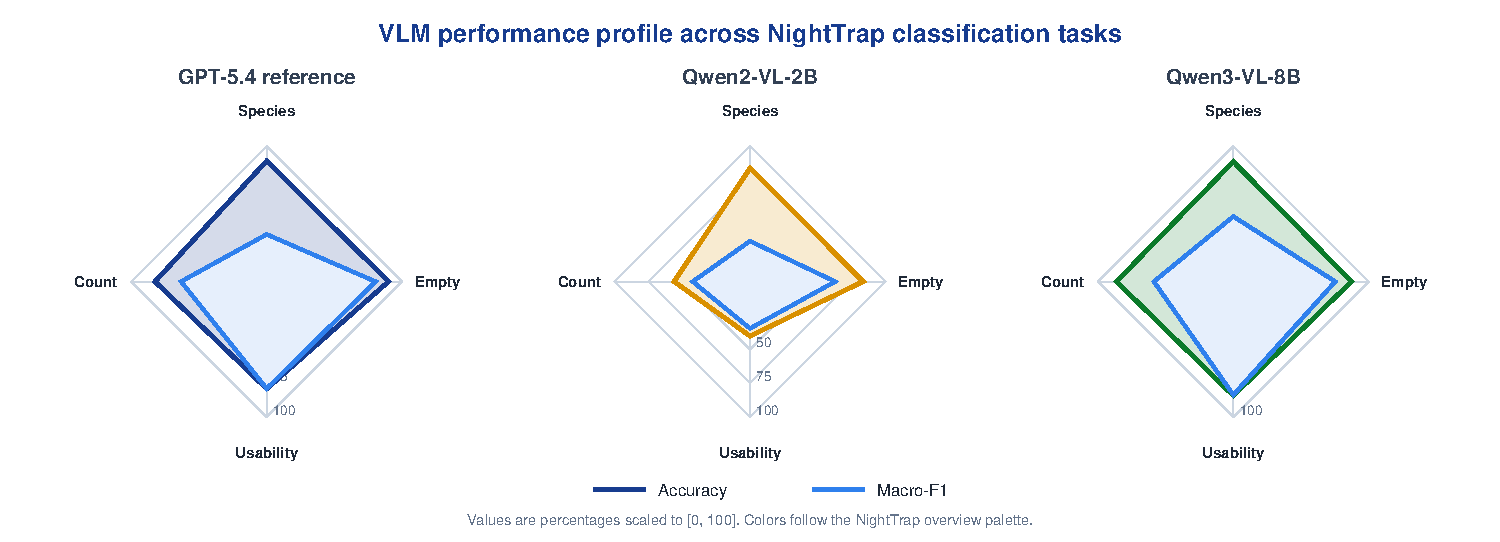
\includegraphics[width=0.90\linewidth]{figures/nighttrap_radar_vlm_grid.pdf}
\caption{VLM capability profiles across the four classification tasks. Accuracy and Macro-F1 are separated to show long-tail gaps.}
\label{fig:radar_vlm_grid}
\end{figure}

\begin{table}[h]
\centering
\caption{Full NightTrap task-set summary, retaining the label distributions from the earlier main-text task table.}
\label{tab:task_definitions_full}
\small
\begin{tabularx}{\textwidth}{lrrrX}
\toprule
Task & Unit & Samples & Sites & Label space / distribution \\
\midrule
Image usability filtering & event & 992 & 361 & insufficient for review decision 600; sufficient for review decision 392 \\
Empty-event filtering & event & 5,236 & 1,170 & nonempty-or-uncertain 4,129; empty false trigger 1,107 \\
Species classification & event & 11,837 & 517 & 55 closed-set species \\
Count-bin classification & event & 22,188 & 212 & 1: 17,374; 2: 2,608; 3--5: 1,683; 6+: 523 \\
Needs-review recommendation & event & 983 & 346 & needs\_review=0: 140; needs\_review=1: 843 \\
\bottomrule
\end{tabularx}
\end{table}

\begin{table*}[h]
\centering
\caption{Needs-review label rubric. The deployed Task 5 target is binary: \texttt{routine} maps to \texttt{needs\_review=0}, and \texttt{review} maps to \texttt{needs\_review=1}. This is a review-assistance label, not a biological novelty label.}
\label{tab:needs_review_rubric}
\scriptsize
\setlength{\tabcolsep}{3pt}
\resizebox{\textwidth}{!}{%
\begin{tabular}{p{2.2cm}p{3.1cm}p{3.0cm}p{3.1cm}p{3.2cm}p{1.4cm}}
\toprule
Benchmark label & Decision meaning & Visible evidence & Site/context condition & Example & Binary mapping \\
\midrule
\texttt{routine} & Image-usable animal event that can be deprioritized under benchmark rules. & Animal is visible and evidence is sufficient for ordinary review. & Allowed site and season context do not indicate a review need. & Common deer, zebra, or similar event at a site where that taxon is routinely observed. & \texttt{0} \\
\texttt{review} & Event should enter the human-review queue because identity, count, or interpretation may need confirmation. & Animal evidence is visible, but the event may be ambiguous, crowded, or worth checking. & Allowed context or visual evidence suggests the event should not be treated as routine. & Ambiguous species appearance, uncertain count, partial body, or event evidence that warrants reviewer confirmation. & \texttt{1} \\
\bottomrule
\end{tabular}
}
\end{table*}


\begin{table*}[h]
\centering
\caption{Label-aware relabeling audit for binary needs-review labels. The benchmark routine/review label was hidden; source species and count labels were shown so the annotator did not need taxonomic expertise. Metrics exclude uncertain rows.}
\label{tab:needs-review-plausibility-audit}
\scriptsize
\setlength{\tabcolsep}{3pt}
\begin{tabular}{lrrrrrrrr}
\toprule
Audit & N & Eval. & Unc. & Agree & $\kappa$ & Routine & Review & Macro \\
\midrule
Label-aware relabeling & 100 & 98 & 2 & 53 & 0.082 & 49.0 & 59.2 & 54.1 \\
\bottomrule
\end{tabular}
\end{table*}


\begin{table*}[t]
\centering
\caption{Ablation and shortcut-check summary. The table reports the main conclusion from each check while keeping the full detailed tables in the appendix. Needs-review rows use the binary \texttt{needs\_review} mapping unless explicitly marked as the 983-event hardset ranking check.}
\label{tab:ablation_diagnostics}
\small
\setlength{\tabcolsep}{4pt}
\resizebox{\textwidth}{!}{%
\begin{tabular}{p{0.19\linewidth}p{0.28\linewidth}p{0.23\linewidth}p{0.22\linewidth}}
\toprule
Diagnostic & Comparison & Main result & Takeaway \\
\midrule
Event representation & First frame vs. three-slot mean on CLIP needs-review split & P@50 is unchanged at 40.00; AUPRC is 30.98 vs. 30.74 & Three image slots do not automatically add useful signal because many events repeat the same frame path. \\
Context shortcut & Image-only, context-lite-only, full context-lite, shuffled context, site-frequency-only & Site-frequency-only reaches P@50=64.00, while context-lite-only has AUROC=60.70 but P@50=18.00 & Site history carries strong priors, so context gains must be treated as shortcut risk unless audited against image evidence. \\
Routine-stress deployment & Qwen3-VL-8B safe auto-pass under recall constraints & Auto-pass is 7.42 at 95\% recall and 3.35 at 98\% recall & Queue ordering is more mature than automatic pass-through; high-recall workload reduction remains small. \\
Imaging mode robustness & Night-color vs. night-IR groups & Qwen3 needs-review P@50 drops from 66.00 on night-color to 52.00 on night-IR & Night imaging mode changes the review recommendation problem and should be reported as a robustness check. \\
Source coverage & Source-wise breakdowns for classification and needs-review & Count-bin is Snapshot Serengeti-only; other tasks vary by source and site composition & Source heterogeneity is part of the benchmark rather than noise to hide. \\
MegaDetector-assisted empty pool & 100-item human audit from the detector-assisted pool & 90 evaluable rows: 53 TP, 4 FP, 32 TN, and 1 FN & Detector-assisted construction is useful infrastructure, but this audit quantifies risk rather than proving detector-independent reliability. \\
\bottomrule
\end{tabular}
}
\end{table*}


\begin{table}[h]
\centering
\caption{Baseline suite retained for reproducibility. All listed rows have corresponding reported or check artifacts unless noted as exploratory.}
\label{tab:baselines}
\small
\begin{tabularx}{\textwidth}{YYY}
\toprule
Baseline & Purpose & Status \\
\midrule
Majority baseline & Lower bound for classification and needs-review decisions & Available for main tables \\
Random-score baseline & Expected queue enrichment under random ranking & Available for needs-review ranking \\
Rule-only baseline & Context-only rule baseline for Input Stress-Test queue-ordering checks & Available for Input Stress-Test check \\
Context Only baseline & Tests whether site context alone solves the review task & Available for Input Stress-Test check \\
CLIP / DINOv2 linear probe & Supervised representation baseline & CLIP available for usability/empty/species/count and needs-review ranker variants; DINOv2 full-frame and detector-crop species linear classifiers available in appendix artifacts \\
ViT / ConvNeXt fine-tuned & Strong supervised image baseline & ViT-B/16 and ConvNeXt-Tiny full-frame fine-tunes available for usability, empty, species, and count; no needs-review fine-tune is reported \\
MegaDetector threshold / detector+classifier & Empty-filtering detector baseline & Empty threshold baseline, detector-assisted empty-pool audit manifest, and 100-item human audit available; CLIP and DINOv2 detector-crop species baselines available with full-frame fallback \\
Qwen2-VL-2B & Open-source VLM baseline & Available for reported tables \\
Qwen3-VL-8B & Open-source VLM baseline & Available for reported tables \\
NVILA-8B & Tuned multimodal comparison / locally adapted VLM & Exploratory appendix comparison; not counted as a supervised NightTrap vision classifier \\
GPT-5.x & Closed-source VLM reference & Exploratory / appendix only \\
\bottomrule
\end{tabularx}
\end{table}

The checked NVILA-8B checkpoint is initialized from a pretrained NVILA/NVILA-Lite model and adapted on AnimalLLaMA data. Its SigLIP/ViT-style vision tower is frozen, and the checked configuration also freezes the multimodal projector. We therefore report NVILA as a locally SFT-adapted multimodal comparison, not as a fine-tuned ConvNeXt/ViT supervised baseline trained on NightTrap splits. Separate full-frame ViT-B/16 and ConvNeXt-Tiny fine-tunes are now available as appendix baselines for usability, empty, species, and count classification; they are not needs-review ranking models.

\begin{table*}[h]
\centering
\caption{Supervised baseline status table. Rows marked available have corresponding result files; no task-specific ViT/ConvNeXt needs-review fine-tune is reported.}
\label{tab:supervised_baseline_status}
\scriptsize
\setlength{\tabcolsep}{3pt}
\begin{tabularx}{\textwidth}{YYYYYY}
\toprule
Model & Training data & Input & Task coverage & Metrics & Status \\
\midrule
CLIP linear probe & NightTrap train split per task & Mean-pooled CLIP embeddings from first/middle/last images & Usability, empty, species, count, needs-review & Accuracy, Macro-F1; AUROC/AUPRC/P@K for needs-review & Available for usability/empty/species/count and CLIP-only needs-review ranker variant \\
ViT / ConvNeXt fine-tuned & NightTrap train split per task & Primary full-frame event image & Species, count, empty, usability & Accuracy, Macro-F1, per-class F1 & ViT-B/16 and ConvNeXt-Tiny fine-tunes available in \path{*_finetune_*_v1/}; needs-review fine-tuning is not reported \\
MegaDetector threshold & Empty-filtering train/dev split for threshold selection & Detector confidence over event images & Empty-event filtering & Accuracy, Macro-F1, per-class F1; human audit FP/FN & Not reported as detector-independent performance; 100-item stratified human audit is available \\
Detector+classifier & Detector crops from NightTrap train split & Animal crops plus full-frame fallback for events without usable boxes & Species; optional empty verification & Accuracy, Macro-F1, per-class F1, coverage & Available for CLIP detector-crop kNN, CLIP detector-crop linear, DINOv2 detector-crop kNN, and DINOv2 detector-crop linear; task-specific ViT/ConvNeXt fine-tunes are full-frame baselines rather than crop-specific detector classifiers \\
DINOv2/CLIP kNN and linear retrieval & NightTrap train/dev/test crop manifest & Frozen crop or full-frame embeddings plus kNN or linear classifier & Species; optional count support & Accuracy, Macro-F1, per-class F1, coverage & CLIP crop kNN available in \path{detector_crop_retrieval_v1/}; CLIP crop linear in \path{detector_crop_clip_linear_v1/}; DINOv2 crop kNN in \path{detector_crop_dinov2_knn_v1/}; DINOv2 crop linear in \path{detector_crop_dinov2_linear_v1/}; DINOv2 full-frame linear in \path{fullframe_dinov2_linear_species_v1/} \\
CLIP+Context supervised ranker & Needs-review train/dev/test split & CLIP event embedding plus allowed context features & Needs-review recommendation & AUROC, AUPRC, P@K, Enrichment@K, safe auto-pass & Available for Visual Only, Context Only, CLIP+Context, context sensitivity logistic variants, and clean XGBoost/LightGBM tree variants; no task-specific ViT/ConvNeXt needs-review fine-tune is reported \\
\bottomrule
\end{tabularx}
\end{table*}

\begin{table}[h]
\centering
\caption{Species representation baselines with detector-crop coverage. All rows evaluate the full 1,775-event species test set. Detector-crop rows use MegaDetector boxes when available and full-frame fallback otherwise.}
\label{tab:detector_crop_species}
\small
\begin{tabular}{lrrrr}
\toprule
Baseline & N & Box coverage & Accuracy & Macro-F1 \\
\midrule
CLIP full-frame linear probe & 1,775 & n/a & 65.30 & 35.58 \\
DINOv2 full-frame linear probe & 1,775 & n/a & 74.03 & 39.50 \\
CLIP detector-crop kNN + fallback & 1,775 & 36.79 & 43.72 & 18.38 \\
CLIP detector-crop linear + fallback & 1,775 & 36.79 & 48.28 & 26.37 \\
DINOv2 detector-crop kNN + fallback & 1,775 & 36.79 & 52.90 & 28.83 \\
DINOv2 detector-crop linear + fallback & 1,775 & 36.79 & 56.06 & 31.15 \\
ViT-B/16 fine-tune & 1,775 & n/a & 57.97 & 24.88 \\
\bottomrule
\end{tabular}
\end{table}


\input{results/nighttrap_tables/table_species_candidate_alignment_v1}

\begin{table*}[h]
\centering
\caption{Supervised full-frame fine-tuning baselines for the four classification tasks. All rows use the primary event image and the frozen NightTrap train/dev/test split for that task.}
\label{tab:supervised_finetune_v1}
\scriptsize
\setlength{\tabcolsep}{3pt}
\resizebox{\textwidth}{!}{%
\begin{tabular}{llrrrll}
\toprule
Model & Task & Test N & Accuracy & Macro-F1 & Training setting & Split \\
\midrule
ViT-B/16 fine-tune & Image usability & 133 & 82.71 & 81.78 & ImageNet init; primary full-frame; AdamW lr $2{\times}10^{-5}$; 2 epochs; batch 16; seed 42 & 720/139/133 train/dev/test \\
ViT-B/16 fine-tune & Empty-event & 785 & 82.68 & 75.10 & ImageNet init; primary full-frame; AdamW lr $2{\times}10^{-5}$; 2 epochs; batch 16; seed 42 & 3,665/786/785 train/dev/test \\
ViT-B/16 fine-tune & Species & 1,775 & 57.97 & 24.88 & ImageNet init; primary full-frame; AdamW lr $2{\times}10^{-5}$; 2 epochs; batch 16; seed 42 & 8,286/1,776/1,775 train/dev/test \\
ViT-B/16 fine-tune & Count-bin & 3,328 & 65.93 & 42.34 & ImageNet init; primary full-frame; AdamW lr $2{\times}10^{-5}$; 2 epochs; batch 16; seed 42 & 15,532/3,328/3,328 train/dev/test \\
ConvNeXt-Tiny fine-tune & Image usability & 133 & 75.94 & 73.41 & ImageNet init; primary full-frame; AdamW lr $2{\times}10^{-5}$; 2 epochs; batch 16; seed 42 & 720/139/133 train/dev/test \\
ConvNeXt-Tiny fine-tune & Empty-event & 785 & 87.13 & 80.13 & ImageNet init; primary full-frame; AdamW lr $2{\times}10^{-5}$; 2 epochs; batch 16; seed 42 & 3,665/786/785 train/dev/test \\
ConvNeXt-Tiny fine-tune & Species & 1,775 & 57.35 & 21.34 & ImageNet init; primary full-frame; AdamW lr $2{\times}10^{-5}$; 2 epochs; batch 16; seed 42 & 8,286/1,776/1,775 train/dev/test \\
ConvNeXt-Tiny fine-tune & Count-bin & 3,328 & 77.07 & 59.70 & ImageNet init; primary full-frame; AdamW lr $2{\times}10^{-5}$; 2 epochs; batch 16; seed 42 & 15,532/3,328/3,328 train/dev/test \\
\bottomrule
\end{tabular}
}
\end{table*}


\input{results/nighttrap_tables/table_convnext_species_convergence_v2}

\begin{table*}[h]
\centering
\caption{Species baselines by inferred night imaging mode. Mode labels are joined from the sensor-context asset inventory by primary image path; missing joins remain unknown.}
\label{tab:species_imaging_breakdown_v1}
\small
\begin{tabular}{llrrr}
\toprule
Model & Imaging mode & N & Accuracy & Macro-F1 \\
\midrule
CLIP full-frame linear & night\_color & 246 & 79.67 & 24.46 \\
CLIP full-frame linear & night\_ir & 1,450 & 63.93 & 22.47 \\
CLIP full-frame linear & night\_lowlight & 75 & 45.33 & 9.65 \\
CLIP full-frame linear & night\_white\_flash & 4 & 50.00 & 2.04 \\
CLIP crop kNN & night\_color & 246 & 63.41 & 15.22 \\
CLIP crop kNN & night\_ir & 1,450 & 39.79 & 10.96 \\
CLIP crop kNN & night\_lowlight & 75 & 54.67 & 11.52 \\
CLIP crop kNN & night\_white\_flash & 4 & 50.00 & 2.17 \\
CLIP crop linear & night\_color & 246 & 70.33 & 18.51 \\
CLIP crop linear & night\_ir & 1,450 & 44.97 & 15.89 \\
CLIP crop linear & night\_lowlight & 75 & 40.00 & 9.51 \\
CLIP crop linear & night\_white\_flash & 4 & 50.00 & 2.00 \\
DINOv2 crop kNN & night\_color & 246 & 73.98 & 22.93 \\
DINOv2 crop kNN & night\_ir & 1,450 & 49.10 & 18.97 \\
DINOv2 crop kNN & night\_lowlight & 75 & 57.33 & 11.06 \\
DINOv2 crop kNN & night\_white\_flash & 4 & 50.00 & 1.82 \\
ViT-B/16 fine-tune & night\_color & 246 & 79.67 & 20.78 \\
ViT-B/16 fine-tune & night\_ir & 1,450 & 56.07 & 17.59 \\
ViT-B/16 fine-tune & night\_lowlight & 75 & 25.33 & 8.30 \\
ViT-B/16 fine-tune & night\_white\_flash & 4 & 25.00 & 1.48 \\
\bottomrule
\end{tabular}
\end{table*}


The imaging-mode join for the species test set covers all 1,775 examples for each reported species baseline using \path{event_sensor_labels.csv}. The available species metadata now separates night-color, night-IR, night-lowlight, and white-flash rows for the species baselines, but night-color support is much smaller than night-IR support, so these rows should be read as a robustness check rather than a balanced cross-mode benchmark.

\subsection{Reproducible Training Details}

For each supervised baseline, the final artifact should include the train/dev/test split path and split policy, image resolution and frame sampling rule, optimizer, learning rate, batch size, number of epochs or solver iterations, random seed, hardware, code path, exact command, checkpoint path when applicable, prediction-file path, and metric script path. Current supervised-baseline execution paths and commands are:
\begin{itemize}
\item \path{CUDA_VISIBLE_DEVICES=4 python3 scripts/nighttrap_ops_v1/92_run_clip_supervised_baselines.py --gpu 4 --tasks empty,species,count}: CLIP linear probes for empty/species/count. Usability uses \path{results/nighttrap_supervised_baselines/clip_linear_probe_v1/usability/}. Outputs: \path{results/nighttrap_supervised_baselines/clip_linear_probe_v1/}.
\item \path{python3 scripts/nighttrap_ops_v1/93_run_megadetector_empty_baseline.py}: MegaDetector threshold baseline for empty-event filtering. Outputs: \path{results/nighttrap_supervised_baselines/megadetector_empty_threshold_v1/}.
\item \path{CUDA_VISIBLE_DEVICES=4 python3 scripts/nighttrap_ops_v1/94_run_needs_review_clip_ranker.py --gpu 4}: CLIP+Context logistic ranker for needs-review recommendation. Outputs: \path{results/nighttrap_supervised_baselines/needs_review_clip_context_ranker_v1/}. Appendix ranker variants reuse the frozen split and embeddings to evaluate Visual Only, Context Only, CLIP+Context, and context sensitivity variants.
\item \path{bash scripts/nighttrap_ops_v1/18_run_end2end_local_model.sh qwen3vl8b results/nighttrap_end2end_smoke_v1/qwen3vl8b_end2end_smoke150 auto}: all-in-one Qwen3-VL-8B smoke check on 150 aligned events. Outputs: \path{results/nighttrap_end2end_smoke_v1/qwen3vl8b_end2end_smoke150/final_parse_and_metric_summary.json} and \path{results/nighttrap_end2end_smoke_v1/qwen3vl8b_end2end_smoke150/binary_needs_review_metrics.json}.
\item \path{CUDA_VISIBLE_DEVICES=4 python3 scripts/nighttrap_ops_v1/101_run_detector_crop_species_baseline.py --gpu 4 --batch-size 128 --k 5}: CLIP detector-crop kNN species baseline using MegaDetector boxes and full-frame fallback for samples without usable boxes. Outputs: \path{results/nighttrap_supervised_baselines/detector_crop_retrieval_v1/}.
\item \path{python3 scripts/nighttrap_ops_v1/102_export_species_baseline_diagnostics.py}: exports per-class F1, confusion matrix, and head/medium/tail checks for the existing CLIP full-frame species linear probe. Outputs: \path{results/nighttrap_supervised_baselines/fullframe_clip_linear_species_v1/}.
\item \path{python3 scripts/nighttrap_ops_v1/103_run_species_representation_extensions.py}: CLIP detector-crop linear classifier and DINOv2 detector-crop kNN species baselines with full-frame fallback. Outputs: \path{results/nighttrap_supervised_baselines/detector_crop_clip_linear_v1/} and \path{results/nighttrap_supervised_baselines/detector_crop_dinov2_knn_v1/}.
\item \path{python3 scripts/nighttrap_ops_v1/107b_run_needs_review_tree_rankers_clean.py}: clean XGBoost and LightGBM needs-review ranker variants on the Ranker Sub-split. The clean context excludes audit flags, audit-only current-species support fields, and site common-species name expansion by default. Outputs: \path{results/nighttrap_supervised_baselines/needs_review_tree_ranker_variants_clean_v1/} and \path{results/nighttrap_tables/table_needs_review_tree_rankers_clean_v1.tex}.
\item \path{CUDA_VISIBLE_DEVICES=3 python3 scripts/nighttrap_ops_v1/108_run_dinov2_species_linear_variants.py --gpu 3 --batch-size 128}: DINOv2 detector-crop linear and full-frame linear species baselines. Outputs: \path{results/nighttrap_supervised_baselines/detector_crop_dinov2_linear_v1/} and \path{results/nighttrap_supervised_baselines/fullframe_dinov2_linear_species_v1/}.
\item \path{CUDA_VISIBLE_DEVICES=3 python3 scripts/nighttrap_ops_v1/104_run_vit_species_finetune.py --epochs 2 --batch-size 16 --num-workers 4}: ViT-B/16 supervised species fine-tune. Outputs: \path{results/nighttrap_supervised_baselines/vit_b16_finetune_species_v1/}.
\item \path{python3 scripts/nighttrap_ops_v1/105_export_species_imaging_breakdown_v1.py}: joins species predictions with sensor-context imaging-mode labels and exports mode/source summaries. Outputs: \path{results/nighttrap_supervised_baselines/species_imaging_breakdown_v1/} and \path{results/nighttrap_tables/table_species_imaging_breakdown_v1.tex}.
\item \path{CUDA_VISIBLE_DEVICES=4 python3 scripts/nighttrap_ops_v1/106_run_image_finetune_baselines.py --gpu 4 --model vit_b16 --task empty/count/usability --epochs 2 --batch-size 16 --num-workers 4}: ViT-B/16 non-species classification fine-tunes. Outputs: \path{results/nighttrap_supervised_baselines/vit_b16_finetune_empty_v1/}, \path{vit_b16_finetune_count_v1/}, and \path{vit_b16_finetune_usability_v1/}.
\item \path{CUDA_VISIBLE_DEVICES=3 python3 scripts/nighttrap_ops_v1/106_run_image_finetune_baselines.py --gpu 3 --model convnext_tiny --task species/empty/count/usability --epochs 2 --batch-size 16 --num-workers 4}: ConvNeXt-Tiny classification fine-tunes. Outputs: \path{results/nighttrap_supervised_baselines/convnext_tiny_finetune_*_v1/}.
\item \path{CUDA_VISIBLE_DEVICES=3 python3 scripts/nighttrap_ops_v1/106_run_image_finetune_baselines.py --gpu 3 --model convnext_tiny --task species --epochs 8 --batch-size 8 --num-workers 4 --lr 2e-5}: ConvNeXt-Tiny species convergence check. Outputs: \path{results/nighttrap_supervised_baselines/convnext_tiny_finetune_species_v2_e8/}. Test Accuracy is 75.38 and Macro-F1 is 36.75; the best dev Macro-F1 occurs at epoch 5.
\end{itemize}

\begin{table}[h]
\centering
\caption{Input and queue-ordering check on the Input Stress-Test ($N=983$). This is a controlled check, not the main needs-review benchmark; the high positive base rate makes enrichment the safer reading of P@50.}
\label{tab:strict983}
\small
\begin{tabular}{llrrrrr}
\toprule
Model & Setting & N & Base & P@50 & E@50 & NDCG@50 \\
\midrule
Rule-only & Context Only & 983 & 0.858 & 0.26 & 0.30 & 0.560 \\
Qwen2-VL-2B & Visual Only & 983 & 0.858 & 0.40 & 0.47 & 0.614 \\
Qwen2-VL-2B & Context Only & 983 & 0.858 & 0.14 & 0.16 & 0.513 \\
Qwen2-VL-2B & Combined & 983 & 0.858 & 0.54 & 0.63 & 0.638 \\
Qwen3-VL-8B & Visual Only & 983 & 0.858 & 0.58 & 0.68 & 0.637 \\
Qwen3-VL-8B & Context Only & 983 & 0.858 & 0.38 & 0.44 & 0.620 \\
Qwen3-VL-8B & Combined & 983 & 0.858 & 0.66 & 0.77 & 0.762 \\
\bottomrule
\end{tabular}
\end{table}

\begin{table*}[h]
\centering
\caption{Original three-level Input Stress-Test check. All rows use the same A/B/C label space and exclude species, rarity, novelty, frequency-band, and seasonality shortcut fields. This check is retained to evaluate queue ordering, while the main Task 5 target remains binary.}
\label{tab:threeway_diagnostic}
\small
\setlength{\tabcolsep}{6pt}
\begin{tabular}{llccccc}
\toprule
Model & Input setting & Acc. & Macro-F1 & P@25 & P@50 & NDCG@50 \\
\midrule
Rule-only & Context Only & 53.00 & 23.09 & 20.00 & 26.00 & 56.00 \\
Qwen3-VL-8B & Visual Only & 48.22 & 24.43 & 56.00 & 58.00 & 63.74 \\
Qwen3-VL-8B & Context Only & 53.00 & 23.12 & 48.00 & 38.00 & 62.03 \\
Qwen3-VL-8B & Combined & 46.29 & 28.87 & 60.00 & 66.00 & 76.18 \\
Qwen2-VL-2B & Visual Only & 52.80 & 23.04 & 44.00 & 40.00 & 61.36 \\
Qwen2-VL-2B & Context Only & 14.24 & 8.31 & 4.00 & 14.00 & 51.25 \\
Qwen2-VL-2B & Combined & 39.27 & 32.97 & 60.00 & 54.00 & 63.81 \\
NVILA-8B$^{\S}$ & Combined & 40.18 & 31.96 & 64.00 & 78.00 & 77.89 \\
GPT-5.4$^{\dagger}$ & Combined & 59.67 & 43.69 & 92.00 & 52.00 & 73.42 \\
GPT-5.2$^{\ddagger}$ & Combined & 58.65 & 42.95 & 76.00 & 38.00 & 72.40 \\
\bottomrule
\end{tabular}
\vspace{0.25em}
\begin{minipage}{0.97\linewidth}
\footnotesize
$^{\S}$ NVILA-8B is a locally adapted NVILA-family VLM with a frozen SigLIP/ViT-style vision tower; it is shown as a tuned multimodal comparison, not as a NightTrap-supervised vision classifier. $^{\dagger,\ddagger}$ GPT rows are closed-source reference rows.
\end{minipage}
\end{table*}

\begin{table*}[h]
\centering
\caption{All-in-one end-to-end smoke check on 150 aligned events. The binary needs-review target maps \texttt{review} and \texttt{priority\_review} to \texttt{needs\_review}. This is a diagnostic check rather than the main comparison, because the subset contains image-usable, nonempty animal events by construction.}
\label{tab:end2end_smoke}
\scriptsize
\setlength{\tabcolsep}{3.2pt}
\begin{tabular}{lrrrrrrrrrr}
\toprule
Model & N & Pos. base & Species exact & Acc. & Macro-F1 & AUROC & AUPRC & P@50 & E@50 & NR recall \\
\midrule
Qwen3-VL-8B & 150 & 63.33 & 12.00 & 42.67 & 39.93 & 54.11 & 64.87 & 72.00 & 1.14 & 16.84 \\
\bottomrule
\end{tabular}
\vspace{0.25em}
\begin{minipage}{0.97\linewidth}
\footnotesize
Acc., Macro-F1, AUROC, AUPRC, P@50, and NR recall are reported for the collapsed binary needs-review target. E@50 is enrichment over the positive base rate. Species exact is included to show one major failure point inside the combined output.
\end{minipage}
\end{table*}

\begin{table}[h]
\centering
\caption{Bootstrap confidence intervals for selected Input Stress-Test rows.}
\label{tab:ci}
\small
\begin{tabular}{llccc}
\toprule
Model & Setting & P@50 [95\% CI] & NDCG@50 [95\% CI] & Macro-F1 [95\% CI] \\
\midrule
Rule-only & Context Only & 0.26 [0.14, 0.40] & 0.560 [0.482, 0.647] & 0.231 [0.221, 0.240] \\
Qwen3-VL-8B & Visual Only & 0.58 [0.44, 0.72] & 0.637 [0.510, 0.789] & 0.244 [0.226, 0.262] \\
Qwen3-VL-8B & Context Only & 0.38 [0.26, 0.54] & 0.620 [0.505, 0.714] & 0.231 [0.221, 0.240] \\
Qwen3-VL-8B & Combined & 0.66 [0.48, 0.76] & 0.762 [0.615, 0.855] & 0.289 [0.262, 0.315] \\
\bottomrule
\end{tabular}
\end{table}

\input{results/nighttrap_tables/table_main_classification_ci_v1}

\input{results/nighttrap_tables/table_task5_bootstrap_ci_v1}

\begin{table*}[h]
\centering
\caption{Full event representation analysis for needs-review recommendation using a CLIP logistic probe. Auto-pass is reported at 95\% needs-review recall.}
\label{tab:event_rep_ablation_full}
\small
\setlength{\tabcolsep}{3pt}
\resizebox{\textwidth}{!}{%
\begin{tabular}{lrrrrrrrrrr}
\toprule
Representation & N & Base & AUROC & AUPRC & Macro-F1 & P@50 & P@100 & E@50 & E@100 & AP@95R \\
\midrule
first-frame-only & 913 & 0.253 & 0.549 & 0.310 & 0.505 & 0.400 & 0.320 & 1.581$\times$ & 1.265$\times$ & 4.38\% \\
middle-frame-only & 913 & 0.253 & 0.536 & 0.308 & 0.485 & 0.380 & 0.390 & 1.502$\times$ & 1.541$\times$ & 6.13\% \\
last-frame-only & 913 & 0.253 & 0.553 & 0.302 & 0.502 & 0.340 & 0.320 & 1.344$\times$ & 1.265$\times$ & 5.91\% \\
three-slot mean & 913 & 0.253 & 0.546 & 0.307 & 0.497 & 0.400 & 0.350 & 1.581$\times$ & 1.383$\times$ & 5.48\% \\
unique-frame-only subset & 281 & 0.263 & 0.492 & 0.290 & 0.490 & 0.300 & 0.270 & 1.139$\times$ & 1.025$\times$ & 5.69\% \\
duplicate-only subset & 632 & 0.248 & 0.570 & 0.319 & 0.500 & 0.380 & 0.360 & 1.530$\times$ & 1.449$\times$ & 4.75\% \\
\\
\bottomrule
\end{tabular}
}
\end{table*}

\begin{table*}[h]
\centering
\caption{Calibration checks for needs-review scores. Qwen3 scores are computed from frozen choice probabilities by summing the probabilities assigned to needs-review choices; CLIP/context-lite scores are logistic probabilities on its frozen 913-event split. ECE uses ten equal-width score bins.}
\label{tab:calibration_appendix}
\small
\setlength{\tabcolsep}{4pt}
\begin{tabular}{lrrrrrrr}
\toprule
Model & N & Base & AUROC & AUPRC & Brier & ECE & AP@95R \\
\midrule
Qwen3-VL-8B full context-lite & 6000 & 30.00 & 57.88 & 38.44 & 0.538 & 0.543 & 7.42 \\
CLIP/context-lite logistic ranker & 913 & 25.30 & 55.98 & 29.72 & 0.360 & 0.348 & 8.43 \\
\bottomrule
\end{tabular}
\vspace{0.25em}
\begin{minipage}{0.95\linewidth}
\footnotesize These checks are computed from frozen scores and do not introduce a new model run. The Qwen3 probabilities are not a separately calibrated binary head, so they should be used as ranking evidence rather than calibrated deployment probabilities.
\end{minipage}
\end{table*}


\begin{table*}[h]
\centering
\caption{Full context shortcut check for needs-review recommendation on the Ranker Sub-split.}
\label{tab:context_shortcut_full}
\small
\setlength{\tabcolsep}{4pt}
\begin{tabular}{lrrrrrrrr}
\toprule
Setting & N & AUROC & AUPRC & Macro-F1 & P@50 & P@100 & E@50 & NDCG@100 \\
\midrule
image-only & 913 & 0.546 & 0.307 & 0.497 & 0.400 & 0.350 & 1.581$\times$ & 0.366 \\
context-lite-only & 913 & 0.607 & 0.324 & 0.514 & 0.180 & 0.430 & 0.711$\times$ & 0.348 \\
full context-lite & 913 & 0.560 & 0.297 & 0.497 & 0.320 & 0.330 & 1.265$\times$ & 0.313 \\
shuffled-context & 913 & 0.531 & 0.286 & 0.496 & 0.360 & 0.310 & 1.423$\times$ & 0.322 \\
site-frequency-only & 913 & 0.569 & 0.353 & 0.459 & 0.640 & 0.490 & 2.530$\times$ & 0.510 \\
rule-only & 913 & 0.450 & 0.228 & 0.457 & 0.140 & 0.180 & 0.553$\times$ & 0.186 \\
\\
\bottomrule
\end{tabular}
\end{table*}

\begin{table*}[h]
\centering
\caption{Context-lite sensitivity on the frozen 913-event needs-review split. Site-frequency-only is a stress-test prior, not the deployed context-lite input. Values are percentages except enrichment.}
\label{tab:context_sensitivity}
\scriptsize
\setlength{\tabcolsep}{3pt}
\begin{tabular}{lrrrrrrrr}
\toprule
Setting & N & AUROC & AUPRC & Macro-F1 & P@50 & P@100 & E@50 & NDCG@100 \\
\midrule
image-only & 913 & 54.63 & 30.74 & 49.74 & 40.00 & 35.00 & 1.58$\times$ & 36.62 \\
full context-lite & 913 & 55.98 & 29.72 & 49.65 & 32.00 & 33.00 & 1.26$\times$ & 31.32 \\
no species-history & 913 & 48.27 & 25.01 & 44.83 & 32.00 & 28.00 & 1.26$\times$ & 31.02 \\
season-only & 913 & 48.27 & 25.01 & 44.83 & 32.00 & 28.00 & 1.26$\times$ & 31.02 \\
site-history without species names & 913 & 54.72 & 28.62 & 47.37 & 28.00 & 27.00 & 1.11$\times$ & 31.28 \\
coarse site-frequency only & 913 & 53.30 & 28.21 & 47.56 & 38.00 & 31.00 & 1.50$\times$ & 39.65 \\
site-frequency-only stress-test prior & 913 & 56.94 & 35.31 & 45.92 & 64.00 & 49.00 & 2.53$\times$ & 51.03 \\
shuffled-context & 913 & 53.07 & 28.64 & 49.65 & 36.00 & 31.00 & 1.42$\times$ & 32.24 \\
\bottomrule
\end{tabular}
\end{table*}


\begin{table*}[h]
\centering
\caption{Needs-review ranker variants on the frozen 913-event CLIP split. All variants use the same site-disjoint split, label mapping, base rate, and score direction. Values are percentages except enrichment.}
\label{tab:ranker_variants}
\scriptsize
\setlength{\tabcolsep}{3pt}
\begin{tabular}{lrrrrrrrr}
\toprule
Setting & N & AUROC & AUPRC & Macro-F1 & P@50 & P@100 & E@50 & AP@95R \\
\midrule
CLIP-only logistic & 913 & 54.63 & 30.74 & 49.74 & 40.00 & 35.00 & 1.58$\times$ & 5.48 \\
context-lite-only logistic & 913 & 60.70 & 32.42 & 51.38 & 18.00 & 43.00 & 0.71$\times$ & 7.34 \\
CLIP+context-lite logistic & 913 & 55.98 & 29.72 & 49.65 & 32.00 & 33.00 & 1.26$\times$ & 8.43 \\
full context-lite without species history & 913 & 48.27 & 25.01 & 44.83 & 32.00 & 28.00 & 1.26$\times$ & 5.26 \\
season-only & 913 & 48.27 & 25.01 & 44.83 & 32.00 & 28.00 & 1.26$\times$ & 5.26 \\
site history without species names & 913 & 54.72 & 28.62 & 47.37 & 28.00 & 27.00 & 1.11$\times$ & 10.51 \\
coarse site-frequency only & 913 & 53.30 & 28.21 & 47.56 & 38.00 & 31.00 & 1.50$\times$ & 12.38 \\
site-frequency-only stress-test prior & 913 & 56.94 & 35.31 & 45.92 & 64.00 & 49.00 & 2.53$\times$ & 10.95 \\
shuffled-context logistic & 913 & 53.07 & 28.64 & 49.65 & 36.00 & 31.00 & 1.42$\times$ & 4.71 \\
\bottomrule
\end{tabular}
\vspace{0.25em}
\begin{minipage}{0.95\linewidth}
\footnotesize These are lightweight logistic variants over frozen CLIP embeddings and allowed context fields. They are check baselines, not new VLM runs.
\end{minipage}
\end{table*}


\begin{table*}[h]
\centering
\caption{Clean tree-based needs-review ranker variants on the frozen 913-event CLIP/context-lite split. Clean context-lite excludes audit flags, audit-only current-species support fields, and site common-species name expansion by default. Values are percentages except enrichment.}
\label{tab:needs_review_tree_rankers_clean}
\scriptsize
\setlength{\tabcolsep}{3pt}
\begin{tabular}{lrrrrrrrr}
\toprule
Setting & N & AUROC & AUPRC & Macro-F1 & P@50 & P@100 & E@50 & AP@95R \\
\midrule
xgboost image-only & 913 & 58.70 & 35.07 & 44.79 & 56.00 & 45.00 & 2.21$\times$ & 3.40 \\
xgboost clean-context-lite-only & 913 & 56.99 & 29.34 & 51.67 & 30.00 & 33.00 & 1.19$\times$ & 10.62 \\
xgboost CLIP+clean-context-lite & 913 & 60.08 & 31.70 & 45.98 & 30.00 & 39.00 & 1.19$\times$ & 10.41 \\
lightgbm image-only & 913 & 58.43 & 35.80 & 44.44 & 54.00 & 46.00 & 2.13$\times$ & 4.27 \\
lightgbm clean-context-lite-only & 913 & 60.88 & 29.30 & 47.90 & 22.00 & 22.00 & 0.87$\times$ & 13.03 \\
lightgbm CLIP+clean-context-lite & 913 & 59.01 & 31.09 & 45.93 & 32.00 & 37.00 & 1.26$\times$ & 10.84 \\
\bottomrule
\end{tabular}
\end{table*}


\begin{table*}[h]
\centering
\caption{Full imaging-mode robustness table. For non-binary tasks, the final metric column repeats Macro-F1; for Needs-review, it reports AUPRC.}
\label{tab:robustness_audits}
\small
\begin{tabular}{lllrrrrr}
\toprule
Mode & Task & Model & N & Acc. & Macro-F1 & P@50 & Metric \\
\midrule
night\_color & Empty-event & CLIP linear probe & 561 & 0.870 & 0.733 & \missingmetric & 0.733 \\
night\_ir & Empty-event & CLIP linear probe & 224 & 0.759 & 0.740 & \missingmetric & 0.740 \\
night\_color & Empty-event & Qwen3-VL-8B & 561 & 0.898 & 0.736 & \missingmetric & 0.736 \\
night\_ir & Empty-event & Qwen3-VL-8B & 224 & 0.808 & 0.751 & \missingmetric & 0.751 \\
night\_color & Needs-review & CLIP/context ranker & 643 & 0.502 & 0.483 & 0.320 & 0.300 \\
night\_ir & Needs-review & CLIP/context ranker & 270 & 0.589 & 0.516 & 0.360 & 0.298 \\
night\_color & Needs-review & Qwen3-VL-8B & 3424 & 0.418 & 0.397 & 0.660 & 0.420 \\
night\_ir & Needs-review & Qwen3-VL-8B & 2575 & 0.373 & 0.372 & 0.520 & 0.335 \\
\\
\bottomrule
\end{tabular}
\end{table*}

\begin{table*}[h]
\centering
\caption{Full source-wise robustness table. Count-bin rows are source-constrained because reliable count labels are available here from Snapshot Serengeti.}
\label{tab:source_breakdown}
\small
\resizebox{\textwidth}{!}{%
\begin{tabular}{lllrrrrr}
\toprule
Source & Task & Model & N & Acc. & Macro-F1 & P@50 & Metric \\
\midrule
Snapshot Serengeti & Count-bin & CLIP linear probe & 3328 & 0.699 & 0.491 & \missingmetric & 0.491 \\
Snapshot Serengeti & Count-bin & Qwen3-VL-8B & 3328 & 0.863 & 0.587 & \missingmetric & 0.587 \\
Caltech Camera Traps & Needs-review & CLIP/context ranker & 218 & 0.583 & 0.527 & 0.380 & 0.317 \\
Idaho Camera Traps & Needs-review & CLIP/context ranker & 52 & 0.615 & 0.424 & 0.200 & 0.271 \\
Snapshot Serengeti & Needs-review & CLIP/context ranker & 462 & 0.472 & 0.469 & 0.340 & 0.337 \\
WCS Camera Traps & Needs-review & CLIP/context ranker & 181 & 0.580 & 0.446 & 0.120 & 0.139 \\
Caltech Camera Traps & Needs-review & Qwen3-VL-8B & 1751 & 0.370 & 0.368 & 0.400 & 0.312 \\
Idaho Camera Traps & Needs-review & Qwen3-VL-8B & 819 & 0.381 & 0.379 & 0.520 & 0.382 \\
Snapshot Serengeti & Needs-review & Qwen3-VL-8B & 2458 & 0.493 & 0.467 & 0.760 & 0.506 \\
WCS Camera Traps & Needs-review & Qwen3-VL-8B & 972 & 0.227 & 0.220 & 0.540 & 0.317 \\
\\
\bottomrule
\end{tabular}
}
\end{table*}

\begin{table}[h]
\centering
\caption{MegaDetector-assisted empty-pool manual-review manifest summary. Bucket-level FP/FN rates are not filled in this manifest table; the completed 100-item human audit is reported separately in Table~\ref{tab:megadetector-independent-audit}.}
\label{tab:megadetector_audit}
\small
\begin{tabular}{lrrrr}
\toprule
Audit bucket & Manifest N & Status & FP rate & FN rate \\
\midrule
empty\_false\_trigger & 131 & 300-item manifest; see Table~\ref{tab:megadetector-independent-audit} & \missingmetric & \missingmetric \\
nonempty\_or\_uncertain & 169 & 300-item manifest; see Table~\ref{tab:megadetector-independent-audit} & \missingmetric & \missingmetric \\
\\
\bottomrule
\end{tabular}
\end{table}

\begin{table*}[h]
\centering
\caption{Independent human audit of MegaDetector empty-event screening on a stratified 100-item subset. Metrics exclude rows labeled uncertain by the annotator; uncertain rows are reported separately and are not counted as detector errors.}
\label{tab:megadetector-independent-audit}
\small
\begin{tabular}{lrrrrrrrrrr}
\toprule
Setting & N & Eval. N & Uncertain & TP & FP & TN & FN & Acc. & Macro-F1 & Prec./Rec. \\
\midrule
Nonempty as positive & 100 & 90 & 10 & 53 & 4 & 32 & 1 & 94.4 & 94.1 & 93.0 / 98.1 \\
\bottomrule
\end{tabular}
\end{table*}


\input{results/nighttrap_tables/table_detector_pool_boundary_v1.tex}

\clearpage
% NeurIPS 2026 Paper Checklist
% Source basis: official NeurIPS 2026 formatting template/checklist.
% This file is intended to be included near the end of the paper with:
%   \newpage
%   % NeurIPS 2026 Paper Checklist
% Source basis: official NeurIPS 2026 formatting template/checklist.
% This file is intended to be included near the end of the paper with:
%   \newpage
%   % NeurIPS 2026 Paper Checklist
% Source basis: official NeurIPS 2026 formatting template/checklist.
% This file is intended to be included near the end of the paper with:
%   \newpage
%   \input{checklist.tex}
%
% The answer macros are normally provided by neurips_2026.sty.
% The fallbacks below make this file more robust if compiled outside that style.

\providecommand{\answerYes}[1][]{\textcolor{blue}{[Yes] #1}}
\providecommand{\answerNo}[1][]{\textcolor{orange}{[No] #1}}
\providecommand{\answerNA}[1][]{\textcolor{gray}{[N/A] #1}}

\section*{NeurIPS Paper Checklist}



\begin{enumerate}

\item {\bf Claims}
\begin{itemize}
    \item[] Question: Do the main claims made in the abstract and introduction accurately reflect the paper's contributions and scope?
    \item[] Answer: \answerYes{}
    \item[] Justification: The abstract and introduction state that NightTrap is a benchmark for night camera-trap review pipelines, with the fifth task fixed as binary needs-review recommendation. The paper also states that safe auto-pass remains limited, matching the reported results.
\end{itemize}

\item {\bf Limitations}
\begin{itemize}
    \item[] Question: Does the paper discuss the limitations of the work performed by the authors?
    \item[] Answer: \answerYes{}
    \item[] Justification: The paper includes a Limitations section covering the scope of needs-review labels, the distinction between the 983-event hardset and 6000-event routine-stress setting, Qwen3 continuous-score calibration, closed-source references, and remaining annotation checks.
\end{itemize}

\item {\bf Theory assumptions and proofs}
\begin{itemize}
    \item[] Question: For each theoretical result, does the paper provide the full set of assumptions and a complete (and correct) proof?
    \item[] Answer: \answerNA{}
    \item[] Justification: The paper introduces a benchmark and empirical evaluation, not theoretical results, theorems, or proofs.
\end{itemize}

\item {\bf Experimental result reproducibility}
\begin{itemize}
    \item[] Question: Does the paper fully disclose all the information needed to reproduce the main experimental results of the paper to the extent that it affects the main claims and/or conclusions of the paper (regardless of whether the code and data are provided or not)?
    \item[] Answer: \answerYes{}
    \item[] Justification: The appendix includes an Artifact, Release, and Reproducibility section with release package, result inventory, run details, and script-to-table mappings for the main results.
\end{itemize}

\item {\bf Open access to data and code}
\begin{itemize}
    \item[] Question: Does the paper provide open access to the data and code, with sufficient instructions to faithfully reproduce the main experimental results, as described in supplemental material?
    \item[] Answer: \answerYes{}
    \item[] Justification: The Hugging Face dataset repository and GitHub code repository are available for anonymous review. The dataset release provides derived benchmark metadata, splits, labels, prompts, result artifacts, Croissant metadata, and access instructions, while the code release provides the smoke test, environment files, paper snapshot, and reproducibility scripts. Raw images are not redistributed; users must obtain them from the upstream sources under the corresponding upstream licenses and access terms.
\end{itemize}

\item {\bf Experimental setting/details}
\begin{itemize}
    \item[] Question: Does the paper specify all the training and test details (e.g., data splits, hyperparameters, how they were chosen, type of optimizer) necessary to understand the results?
    \item[] Answer: \answerYes{}
    \item[] Justification: The experimental setup is described in the main paper, and appendix tables document result inventory, scripts, inputs, outputs, and available run details.
\end{itemize}

\item {\bf Experiment statistical significance}
\begin{itemize}
    \item[] Question: Does the paper report error bars suitably and correctly defined or other appropriate information about the statistical significance of the experiments?
    \item[] Answer: \answerNo{}
    \item[] Justification: Selected bootstrap confidence intervals, calibration diagnostics, and human-audit summaries exist, but not all main rows have uncertainty intervals.
\end{itemize}

\item {\bf Experiments compute resources}
\begin{itemize}
    \item[] Question: For each experiment, does the paper provide sufficient information on the computer resources (type of compute workers, memory, time of execution) needed to reproduce the experiments?
    \item[] Answer: \answerNo{}
    \item[] Justification: The appendix includes a partial compute-resource table. Newly added ViT/ConvNeXt and related baselines have partial records, but older VLM runtime information is incomplete.
\end{itemize}

\item {\bf Code of ethics}
\begin{itemize}
    \item[] Question: Does the research conducted in the paper conform, in every respect, with the NeurIPS Code of Ethics \url{https://neurips.cc/public/EthicsGuidelines}?
    \item[] Answer: \answerYes{}
    \item[] Justification: The paper includes safeguards for data access, anonymization, non-redistribution of restricted raw images, and human-in-the-loop use.
\end{itemize}

\item {\bf Broader impacts}
\begin{itemize}
    \item[] Question: Does the paper discuss both potential positive societal impacts and negative societal impacts of the work performed?
    \item[] Answer: \answerYes{}
    \item[] Justification: The appendix includes a Broader Impacts and Safeguards section covering positive effects, failure risks, sensitive location/species risks, and detector-pool bias.
\end{itemize}

\item {\bf Safeguards}
\begin{itemize}
    \item[] Question: Does the paper describe safeguards that have been put in place for responsible release of data or models that have a high risk for misuse (e.g., pre-trained language models, image generators, or scraped datasets)?
    \item[] Answer: \answerYes{}
    \item[] Justification: The paper describes safeguards including site/location anonymization, license-gated raw-image access, no restricted raw-image redistribution, high-recall safe auto-pass reporting, and a manual audit manifest plus completed 100-item human audit for detector-assisted empty pools.
\end{itemize}

\item {\bf Licenses for existing assets}
\begin{itemize}
    \item[] Question: Are the creators or original owners of assets (e.g., code, data, models), used in the paper, properly credited and are the license and terms of use explicitly mentioned and properly respected?
    \item[] Answer: \answerYes{}
    \item[] Justification: The appendix provides a license and data-access inventory for source datasets and models. NightTrap releases derived metadata, labels, splits, prompts, and code; raw images and model weights are not redistributed and remain governed by upstream provider or model-card terms.
\end{itemize}

\item {\bf New assets}
\begin{itemize}
    \item[] Question: Are new assets introduced in the paper well documented and is the documentation provided alongside the assets?
    \item[] Answer: \answerYes{}
    \item[] Justification: NightTrap releases derived metadata, splits, labels, prompts, Croissant metadata, a dataset card, and code, while documenting that raw images are governed by upstream access terms.
\end{itemize}

\item {\bf Crowdsourcing and research with human subjects}
\begin{itemize}
    \item[] Question: For crowdsourcing experiments and research with human subjects, does the paper include the full text of instructions given to participants and screenshots, if applicable, as well as details about compensation (if any)?
    \item[] Answer: \answerYes{}
    \item[] Justification: The appendix includes an English translation of the questionnaire items and an aggregate-response summary. The questionnaire is low-risk aggregate motivation material, does not collect sensitive personal attributes, and is not used to produce benchmark labels or experimental results.
\end{itemize}

\item {\bf Institutional review board (IRB) approvals or equivalent for research with human subjects}
\begin{itemize}
    \item[] Question: Does the paper describe potential risks incurred by study participants, whether such risks were disclosed to the subjects, and whether Institutional Review Board (IRB) approvals (or an equivalent approval/review based on the requirements of your country or institution) were obtained?
    \item[] Answer: \answerNo{}
    \item[] Justification: No IRB approval is claimed. The questionnaire was low-risk and non-interventional, and it was used only as aggregate motivation rather than for benchmark labels or experimental results.
\end{itemize}

\item {\bf Declaration of LLM usage}
\begin{itemize}
    \item[] Question: Does the paper describe the usage of LLMs if it is an important, original, or non-standard component of the core methods in this research? Note that if the LLM is used only for writing, editing, or formatting purposes and does not impact the core methodology, scientific rigor, or originality of the research, declaration is not required.
    \item[] Answer: \answerYes{}
    \item[] Justification: The appendix declares that VLMs are experimental subjects in the benchmark. Any LLM assistance for writing or editing did not generate benchmark labels or experimental results.
\end{itemize}

\end{enumerate}

%
% The answer macros are normally provided by neurips_2026.sty.
% The fallbacks below make this file more robust if compiled outside that style.

\providecommand{\answerYes}[1][]{\textcolor{blue}{[Yes] #1}}
\providecommand{\answerNo}[1][]{\textcolor{orange}{[No] #1}}
\providecommand{\answerNA}[1][]{\textcolor{gray}{[N/A] #1}}

\section*{NeurIPS Paper Checklist}



\begin{enumerate}

\item {\bf Claims}
\begin{itemize}
    \item[] Question: Do the main claims made in the abstract and introduction accurately reflect the paper's contributions and scope?
    \item[] Answer: \answerYes{}
    \item[] Justification: The abstract and introduction state that NightTrap is a benchmark for night camera-trap review pipelines, with the fifth task fixed as binary needs-review recommendation. The paper also states that safe auto-pass remains limited, matching the reported results.
\end{itemize}

\item {\bf Limitations}
\begin{itemize}
    \item[] Question: Does the paper discuss the limitations of the work performed by the authors?
    \item[] Answer: \answerYes{}
    \item[] Justification: The paper includes a Limitations section covering the scope of needs-review labels, the distinction between the 983-event hardset and 6000-event routine-stress setting, Qwen3 continuous-score calibration, closed-source references, and remaining annotation checks.
\end{itemize}

\item {\bf Theory assumptions and proofs}
\begin{itemize}
    \item[] Question: For each theoretical result, does the paper provide the full set of assumptions and a complete (and correct) proof?
    \item[] Answer: \answerNA{}
    \item[] Justification: The paper introduces a benchmark and empirical evaluation, not theoretical results, theorems, or proofs.
\end{itemize}

\item {\bf Experimental result reproducibility}
\begin{itemize}
    \item[] Question: Does the paper fully disclose all the information needed to reproduce the main experimental results of the paper to the extent that it affects the main claims and/or conclusions of the paper (regardless of whether the code and data are provided or not)?
    \item[] Answer: \answerYes{}
    \item[] Justification: The appendix includes an Artifact, Release, and Reproducibility section with release package, result inventory, run details, and script-to-table mappings for the main results.
\end{itemize}

\item {\bf Open access to data and code}
\begin{itemize}
    \item[] Question: Does the paper provide open access to the data and code, with sufficient instructions to faithfully reproduce the main experimental results, as described in supplemental material?
    \item[] Answer: \answerYes{}
    \item[] Justification: The Hugging Face dataset repository and GitHub code repository are available for anonymous review. The dataset release provides derived benchmark metadata, splits, labels, prompts, result artifacts, Croissant metadata, and access instructions, while the code release provides the smoke test, environment files, paper snapshot, and reproducibility scripts. Raw images are not redistributed; users must obtain them from the upstream sources under the corresponding upstream licenses and access terms.
\end{itemize}

\item {\bf Experimental setting/details}
\begin{itemize}
    \item[] Question: Does the paper specify all the training and test details (e.g., data splits, hyperparameters, how they were chosen, type of optimizer) necessary to understand the results?
    \item[] Answer: \answerYes{}
    \item[] Justification: The experimental setup is described in the main paper, and appendix tables document result inventory, scripts, inputs, outputs, and available run details.
\end{itemize}

\item {\bf Experiment statistical significance}
\begin{itemize}
    \item[] Question: Does the paper report error bars suitably and correctly defined or other appropriate information about the statistical significance of the experiments?
    \item[] Answer: \answerNo{}
    \item[] Justification: Selected bootstrap confidence intervals, calibration diagnostics, and human-audit summaries exist, but not all main rows have uncertainty intervals.
\end{itemize}

\item {\bf Experiments compute resources}
\begin{itemize}
    \item[] Question: For each experiment, does the paper provide sufficient information on the computer resources (type of compute workers, memory, time of execution) needed to reproduce the experiments?
    \item[] Answer: \answerNo{}
    \item[] Justification: The appendix includes a partial compute-resource table. Newly added ViT/ConvNeXt and related baselines have partial records, but older VLM runtime information is incomplete.
\end{itemize}

\item {\bf Code of ethics}
\begin{itemize}
    \item[] Question: Does the research conducted in the paper conform, in every respect, with the NeurIPS Code of Ethics \url{https://neurips.cc/public/EthicsGuidelines}?
    \item[] Answer: \answerYes{}
    \item[] Justification: The paper includes safeguards for data access, anonymization, non-redistribution of restricted raw images, and human-in-the-loop use.
\end{itemize}

\item {\bf Broader impacts}
\begin{itemize}
    \item[] Question: Does the paper discuss both potential positive societal impacts and negative societal impacts of the work performed?
    \item[] Answer: \answerYes{}
    \item[] Justification: The appendix includes a Broader Impacts and Safeguards section covering positive effects, failure risks, sensitive location/species risks, and detector-pool bias.
\end{itemize}

\item {\bf Safeguards}
\begin{itemize}
    \item[] Question: Does the paper describe safeguards that have been put in place for responsible release of data or models that have a high risk for misuse (e.g., pre-trained language models, image generators, or scraped datasets)?
    \item[] Answer: \answerYes{}
    \item[] Justification: The paper describes safeguards including site/location anonymization, license-gated raw-image access, no restricted raw-image redistribution, high-recall safe auto-pass reporting, and a manual audit manifest plus completed 100-item human audit for detector-assisted empty pools.
\end{itemize}

\item {\bf Licenses for existing assets}
\begin{itemize}
    \item[] Question: Are the creators or original owners of assets (e.g., code, data, models), used in the paper, properly credited and are the license and terms of use explicitly mentioned and properly respected?
    \item[] Answer: \answerYes{}
    \item[] Justification: The appendix provides a license and data-access inventory for source datasets and models. NightTrap releases derived metadata, labels, splits, prompts, and code; raw images and model weights are not redistributed and remain governed by upstream provider or model-card terms.
\end{itemize}

\item {\bf New assets}
\begin{itemize}
    \item[] Question: Are new assets introduced in the paper well documented and is the documentation provided alongside the assets?
    \item[] Answer: \answerYes{}
    \item[] Justification: NightTrap releases derived metadata, splits, labels, prompts, Croissant metadata, a dataset card, and code, while documenting that raw images are governed by upstream access terms.
\end{itemize}

\item {\bf Crowdsourcing and research with human subjects}
\begin{itemize}
    \item[] Question: For crowdsourcing experiments and research with human subjects, does the paper include the full text of instructions given to participants and screenshots, if applicable, as well as details about compensation (if any)?
    \item[] Answer: \answerYes{}
    \item[] Justification: The appendix includes an English translation of the questionnaire items and an aggregate-response summary. The questionnaire is low-risk aggregate motivation material, does not collect sensitive personal attributes, and is not used to produce benchmark labels or experimental results.
\end{itemize}

\item {\bf Institutional review board (IRB) approvals or equivalent for research with human subjects}
\begin{itemize}
    \item[] Question: Does the paper describe potential risks incurred by study participants, whether such risks were disclosed to the subjects, and whether Institutional Review Board (IRB) approvals (or an equivalent approval/review based on the requirements of your country or institution) were obtained?
    \item[] Answer: \answerNo{}
    \item[] Justification: No IRB approval is claimed. The questionnaire was low-risk and non-interventional, and it was used only as aggregate motivation rather than for benchmark labels or experimental results.
\end{itemize}

\item {\bf Declaration of LLM usage}
\begin{itemize}
    \item[] Question: Does the paper describe the usage of LLMs if it is an important, original, or non-standard component of the core methods in this research? Note that if the LLM is used only for writing, editing, or formatting purposes and does not impact the core methodology, scientific rigor, or originality of the research, declaration is not required.
    \item[] Answer: \answerYes{}
    \item[] Justification: The appendix declares that VLMs are experimental subjects in the benchmark. Any LLM assistance for writing or editing did not generate benchmark labels or experimental results.
\end{itemize}

\end{enumerate}

%
% The answer macros are normally provided by neurips_2026.sty.
% The fallbacks below make this file more robust if compiled outside that style.

\providecommand{\answerYes}[1][]{\textcolor{blue}{[Yes] #1}}
\providecommand{\answerNo}[1][]{\textcolor{orange}{[No] #1}}
\providecommand{\answerNA}[1][]{\textcolor{gray}{[N/A] #1}}

\section*{NeurIPS Paper Checklist}



\begin{enumerate}

\item {\bf Claims}
\begin{itemize}
    \item[] Question: Do the main claims made in the abstract and introduction accurately reflect the paper's contributions and scope?
    \item[] Answer: \answerYes{}
    \item[] Justification: The abstract and introduction state that NightTrap is a benchmark for night camera-trap review pipelines, with the fifth task fixed as binary needs-review recommendation. The paper also states that safe auto-pass remains limited, matching the reported results.
\end{itemize}

\item {\bf Limitations}
\begin{itemize}
    \item[] Question: Does the paper discuss the limitations of the work performed by the authors?
    \item[] Answer: \answerYes{}
    \item[] Justification: The paper includes a Limitations section covering the scope of needs-review labels, the distinction between the 983-event hardset and 6000-event routine-stress setting, Qwen3 continuous-score calibration, closed-source references, and remaining annotation checks.
\end{itemize}

\item {\bf Theory assumptions and proofs}
\begin{itemize}
    \item[] Question: For each theoretical result, does the paper provide the full set of assumptions and a complete (and correct) proof?
    \item[] Answer: \answerNA{}
    \item[] Justification: The paper introduces a benchmark and empirical evaluation, not theoretical results, theorems, or proofs.
\end{itemize}

\item {\bf Experimental result reproducibility}
\begin{itemize}
    \item[] Question: Does the paper fully disclose all the information needed to reproduce the main experimental results of the paper to the extent that it affects the main claims and/or conclusions of the paper (regardless of whether the code and data are provided or not)?
    \item[] Answer: \answerYes{}
    \item[] Justification: The appendix includes an Artifact, Release, and Reproducibility section with release package, result inventory, run details, and script-to-table mappings for the main results.
\end{itemize}

\item {\bf Open access to data and code}
\begin{itemize}
    \item[] Question: Does the paper provide open access to the data and code, with sufficient instructions to faithfully reproduce the main experimental results, as described in supplemental material?
    \item[] Answer: \answerYes{}
    \item[] Justification: The Hugging Face dataset repository and GitHub code repository are available for anonymous review. The dataset release provides derived benchmark metadata, splits, labels, prompts, result artifacts, Croissant metadata, and access instructions, while the code release provides the smoke test, environment files, paper snapshot, and reproducibility scripts. Raw images are not redistributed; users must obtain them from the upstream sources under the corresponding upstream licenses and access terms.
\end{itemize}

\item {\bf Experimental setting/details}
\begin{itemize}
    \item[] Question: Does the paper specify all the training and test details (e.g., data splits, hyperparameters, how they were chosen, type of optimizer) necessary to understand the results?
    \item[] Answer: \answerYes{}
    \item[] Justification: The experimental setup is described in the main paper, and appendix tables document result inventory, scripts, inputs, outputs, and available run details.
\end{itemize}

\item {\bf Experiment statistical significance}
\begin{itemize}
    \item[] Question: Does the paper report error bars suitably and correctly defined or other appropriate information about the statistical significance of the experiments?
    \item[] Answer: \answerNo{}
    \item[] Justification: Selected bootstrap confidence intervals, calibration diagnostics, and human-audit summaries exist, but not all main rows have uncertainty intervals.
\end{itemize}

\item {\bf Experiments compute resources}
\begin{itemize}
    \item[] Question: For each experiment, does the paper provide sufficient information on the computer resources (type of compute workers, memory, time of execution) needed to reproduce the experiments?
    \item[] Answer: \answerNo{}
    \item[] Justification: The appendix includes a partial compute-resource table. Newly added ViT/ConvNeXt and related baselines have partial records, but older VLM runtime information is incomplete.
\end{itemize}

\item {\bf Code of ethics}
\begin{itemize}
    \item[] Question: Does the research conducted in the paper conform, in every respect, with the NeurIPS Code of Ethics \url{https://neurips.cc/public/EthicsGuidelines}?
    \item[] Answer: \answerYes{}
    \item[] Justification: The paper includes safeguards for data access, anonymization, non-redistribution of restricted raw images, and human-in-the-loop use.
\end{itemize}

\item {\bf Broader impacts}
\begin{itemize}
    \item[] Question: Does the paper discuss both potential positive societal impacts and negative societal impacts of the work performed?
    \item[] Answer: \answerYes{}
    \item[] Justification: The appendix includes a Broader Impacts and Safeguards section covering positive effects, failure risks, sensitive location/species risks, and detector-pool bias.
\end{itemize}

\item {\bf Safeguards}
\begin{itemize}
    \item[] Question: Does the paper describe safeguards that have been put in place for responsible release of data or models that have a high risk for misuse (e.g., pre-trained language models, image generators, or scraped datasets)?
    \item[] Answer: \answerYes{}
    \item[] Justification: The paper describes safeguards including site/location anonymization, license-gated raw-image access, no restricted raw-image redistribution, high-recall safe auto-pass reporting, and a manual audit manifest plus completed 100-item human audit for detector-assisted empty pools.
\end{itemize}

\item {\bf Licenses for existing assets}
\begin{itemize}
    \item[] Question: Are the creators or original owners of assets (e.g., code, data, models), used in the paper, properly credited and are the license and terms of use explicitly mentioned and properly respected?
    \item[] Answer: \answerYes{}
    \item[] Justification: The appendix provides a license and data-access inventory for source datasets and models. NightTrap releases derived metadata, labels, splits, prompts, and code; raw images and model weights are not redistributed and remain governed by upstream provider or model-card terms.
\end{itemize}

\item {\bf New assets}
\begin{itemize}
    \item[] Question: Are new assets introduced in the paper well documented and is the documentation provided alongside the assets?
    \item[] Answer: \answerYes{}
    \item[] Justification: NightTrap releases derived metadata, splits, labels, prompts, Croissant metadata, a dataset card, and code, while documenting that raw images are governed by upstream access terms.
\end{itemize}

\item {\bf Crowdsourcing and research with human subjects}
\begin{itemize}
    \item[] Question: For crowdsourcing experiments and research with human subjects, does the paper include the full text of instructions given to participants and screenshots, if applicable, as well as details about compensation (if any)?
    \item[] Answer: \answerYes{}
    \item[] Justification: The appendix includes an English translation of the questionnaire items and an aggregate-response summary. The questionnaire is low-risk aggregate motivation material, does not collect sensitive personal attributes, and is not used to produce benchmark labels or experimental results.
\end{itemize}

\item {\bf Institutional review board (IRB) approvals or equivalent for research with human subjects}
\begin{itemize}
    \item[] Question: Does the paper describe potential risks incurred by study participants, whether such risks were disclosed to the subjects, and whether Institutional Review Board (IRB) approvals (or an equivalent approval/review based on the requirements of your country or institution) were obtained?
    \item[] Answer: \answerNo{}
    \item[] Justification: No IRB approval is claimed. The questionnaire was low-risk and non-interventional, and it was used only as aggregate motivation rather than for benchmark labels or experimental results.
\end{itemize}

\item {\bf Declaration of LLM usage}
\begin{itemize}
    \item[] Question: Does the paper describe the usage of LLMs if it is an important, original, or non-standard component of the core methods in this research? Note that if the LLM is used only for writing, editing, or formatting purposes and does not impact the core methodology, scientific rigor, or originality of the research, declaration is not required.
    \item[] Answer: \answerYes{}
    \item[] Justification: The appendix declares that VLMs are experimental subjects in the benchmark. Any LLM assistance for writing or editing did not generate benchmark labels or experimental results.
\end{itemize}

\end{enumerate}


\end{document}
